\documentclass[11pt,a4paper,spanish]{book}

\usepackage[spanish]{babel}

\usepackage[utf8]{inputenc}

\usepackage{graphicx}

\usepackage{subcaption}

\usepackage[a4paper,left=3cm,right=2cm,top=3cm,bottom=2cm]{geometry}

\usepackage{url}

\usepackage{lineno}
\linenumbers

\setlength{\parskip}{1.5mm}

\begin{document}

%Empieza la numeración en números romanos
\frontmatter
% Incluimos la carátula
%Observación: Si bien la página del prefacio dice que sea empty, debería
%comenzar allí la numeración. Se sugiere numeración romana. Recomenzar la
%numeración en el primer capítulo de la tesis con numeración arábiga.

\titlepage

\begin{center}
\ \\
\ \\
\vspace{-1cm}


\ \\

\vspace{0.5cm}
{\Large{\bf \sc Universidad Nacional del Comahue}}\\

\ \\
{\Large { \sc Facultad de Informática}}\\

\vspace{-2.5cm}
\mbox{\hspace{-1cm}\includegraphics[width=2.5cm,height=2.5cm]{logos/uncoma.pdf}\hspace{13cm} 
\includegraphics[width=2.5cm,height=2.5cm]{logos/fai.pdf}}


\vspace{6cm}

{\Large {\bf\sc Tesis de Licenciado en Ciencias de la Computación}}\\
\ \\
\ \\
{\LARGE {\bf Un sistema paralelo de visión global para futbol de robots
	orientado al uso educativo}}\\
\vspace{3cm}

{\Large Autor: Cañibano, Rodrigo S.}\\
\vspace{2cm}

{\Large Director: Balladini, Javier}\\
\ \\
{\Large Codirector: Grosclaude, Eduardo}\\

\vfill
{\Large {\sc Neuquén}\hspace{6cm}{\sc Argentina}}\\
\ \\

{\Large 2017}\\

\end{center}

\pagebreak



\ \\
\ \\
\label{pagpref}
\noindent{\LARGE \sc Prefacio}\\
\ \\
\ \\

\ \\

\ \\
\ \\


Esta tesis es presentada como parte de los requisitos finales para optar al
grado académico de {\em Licenciado en Ciencias de la Computación}, otorgado por
la Universidad Nacional del Comahue, y no ha sido presentada previamente para la
obtención de otro título en esta Universidad u otras. La misma es el resultado
de la investigación llevada a cabo en el Departamento de ingeniería de
computadoras de la Facultad de Informática, en el período comprendido entre
Marzo de 2015 y .... de 2017, bajo la dirección de Javier Balladini y la
codirección de Eduardo Grosclaude.

\vspace{3cm}


\ \\
{\flushright Rodrigo S. Cañibano\\
{\sc Facultad de Informática \\
Universidad Nacional del Comahue}\\
{\em Neuquén, .. de .... de 2017.}\\}

\vfill

\begin{center}
%
\framebox{\begin{minipage}[t]{0.9\columnwidth}%
\begin{flushleft}

\includegraphics[scale=0.035]{logos/unc.png}

\vspace{-2cm}
{\large \hspace{5cm}\sc universidad
nacional del comahue} \\
\par\end{flushleft}
\begin{center}
{\large \qquad{}}{ \hspace{2.5cm} Facultad de Informática}
\par\end{center}

\vspace{1cm}

\indent \ \ \ \ \ \ \ \ \ \ \ La presente tesis ha sido aprobada el día ........................., mereciendo la \\
\indent \ \ \ \  \ \ \ \ \ calificación de .............................

\medskip{}

\vspace{1cm}
\end{minipage}}
\end{center}

\pagebreak


% Incluimos la página de resumen
% vim: set spell spelllang=es syntax=tex :
\ \\
\ \\
\label{pagresum}
\noindent{\LARGE \sc Resumen}\\
\ \\
\ \\

\ \\

\ \\

La \emph{RoboCup} (del inglés \emph{Robot World Cup}) es una competencia donde
equipos de robots juegan una versión simplificada del fútbol. Su finalidad es
la de ofrecer un ambiente controlado donde poner a prueba los avances en
distintas áreas de conocimiento como la inteligencia artificial, visión por
computadora y robótica. Existen cinco ligas distintas cuyas características
varían desde la simulación del ambiente y robots, hasta robots humanoides con
visión local, la más antigua de éstas es la liga de tamaño pequeño (también
llamada \emph{SSL} por sus siglas en inglés).

\emph{SSL} utiliza un sistema de visión global compartido por los dos equipos.
El sistema procesa cuadros de vídeo y reporta la posición y orientación de los
robots y la posición de la pelota en cada uno de ellos. En este trabajo se
presenta un nuevo sistema de visión global por computadora alternativo al
utilizado actualmente por la \emph{RoboCup} para la \emph{SSL}, que puede ser
utilizado como herramienta educativa en una asignatura de visión por Computadora
y permite explorar distintas estrategias de paralelización. Se tomo como base el
trabajo realizado en \cite{torres2014} y se le aplicaron conjuntamente dos
estrategias de paralelización. Una de ellas explota el paralelismo dentro de
cada cuadro, dividiendo los cuadros en fragmentos que son procesados de forma
independiente. La otra estrategia se basa en el procesamiento simultáneo de
diferentes cuadros del vídeo.

Se realizó una implementación en OpenMP para C++, basada en plugins para
facilitar su modificación en un ambiente educativo. En un servidor con un
procesador Intel Xeon E5-2630 (6 núcleos y multithreading simultáneo) el
sistema logra una mejora máxima de 5,0x en los FPS procesados mientras el
retardo por cuadro se redujo a menos del 20\%, con respecto a la ejecución del
sistema utilizando un único núcleo (de los 6 disponibles).

\vfill
\pagebreak


% Incluimos la página de resumen en inglés
% vim: set spell spelllang=en syntax=tex :
\ \\
\ \\
\label{pagsumm}
\noindent{\LARGE \sc Abstract}\\
\ \\
\ \\

\ \\

\ \\
\ \\

The \emph{RoboCup} (short for \emph{Robot World Cup}) is a tournament where two
teams play a simplified version of football. Its aim is to provide a platform
where the advances on multiple fields like artificial intelligence, computer
vision, and robotics can be put to a test. The \emph{RoboCup} has five leagues
ranging from simulated robots on a virtual field, up to humanoid robots with
local vision. Its most ancient league is the \emph{Small Size League}, also
called the \emph{SSL}.

On the \emph{SSL} games, the global vision system is shared by both teams. The
system process the video frames and reports the robots' and ball's position and
orientation. We propose an alternative global vision system to that used by the
\emph{RoboCup} for the \emph{SSL} games, that can be used as a learning tool for
computer vision and shared memory parallel programming courses.

For a global vision system to be useful as a learning tool, its detection
algorithms must show a clear conceptual division and be implemented simply so it
can be easily modified (even if it implies a performance loss). Using a base
system, we develop a new system able to efficiently use multiple processing
units and its memory hierarchy. Two parallelization strategies where apply.
The first one applies parallelism inside a frame, dividing the frames into
fragments that are processed independently. The other strategy is based on the
simultaneous precessing of different frames.

The system was implemented using \emph{OpenMP} shared memory programming model
for \emph{C++}. The application's parallelization strategies' parameters can be
tuned to obtain maximum performance for a specific hardware platform. On a
server with an Intel Xeon E5-2630 processor (with 6 processing units and
simultaneous multithreading), we achieve an improvement of 5.42$x$ \emph{FPS},
in comparison to the run using only one processing unit (from the 6 available).
The parallelization strategies can be modified, this can be used to led students
experiment and analyze its results to explain its impact on the system
performance.

\vfill
\pagebreak


\tableofcontents
\listoffigures
%Empieza la numeración en números arábigos
\mainmatter

\chapter{Introducción}

% vim: set spell spelllang=es syntax=tex :

\section{Fútbol de robots}

La \emph{RoboCup} (abreviación del ingles \emph{Robot World Cup}) es una
competencia internacional celebrada desde 1997, donde equipos de robots juegan
una versión simplificada del fútbol. Su finalidad es la de poner a prueba los
avances en distintas áreas de conocimiento como la inteligencia artificial,
visión por computadora y robótica. Existen cinco ligas distintas que van desde
el ambiente y robots simulados a robots humanoides con visión local. De estas,
la mas antigua es la liga de tamaño pequeño (\emph{SSL}, del ingles \emph{Small
Size League}).

Un partido de la \emph{SSL} enfrenta a dos equipos de seis robots, que deben
tener un tamaño menor que un cilindro de 9$cm$ de radio y 15$cm$ de
alto\cite{sslrules2015}. Los robots tienen capacidad de procesamiento reducida,
delegando la toma de decisiones a la computadora de su equipo. Estas a su vez
perciben el ambiente a través de un sistema de visión global centralizado
compartido. Este sistema de visión consta de un conjunto de cámaras montadas
sobre distintas áreas del campo de juego conectadas a una computadora donde se
ejecuta el sistema de visión. El sistema detecta la posición y orientación de
cada uno de los robots y la posición de la pelota, y reporta esta información a
las computadoras que controlan los equipos.

Para poder identificar a cada robot cada robot tiene sobre su parte superior 5
parches de colores. El parche que se encuentra en el centro indica el color del
equipo del robot, los cuatro restantes sirven para identificar al robot dentro
del equipo y su orientación. La pelota de color liso distinto a el de los
parches de los robots, normalmente naranja, ya que contrasta fácilmente con el
verde de la cancha. En la figura \ref{sistemaVG} se presenta un diagrama
mostrando esta estructura.

\begin{figure}[!h]

	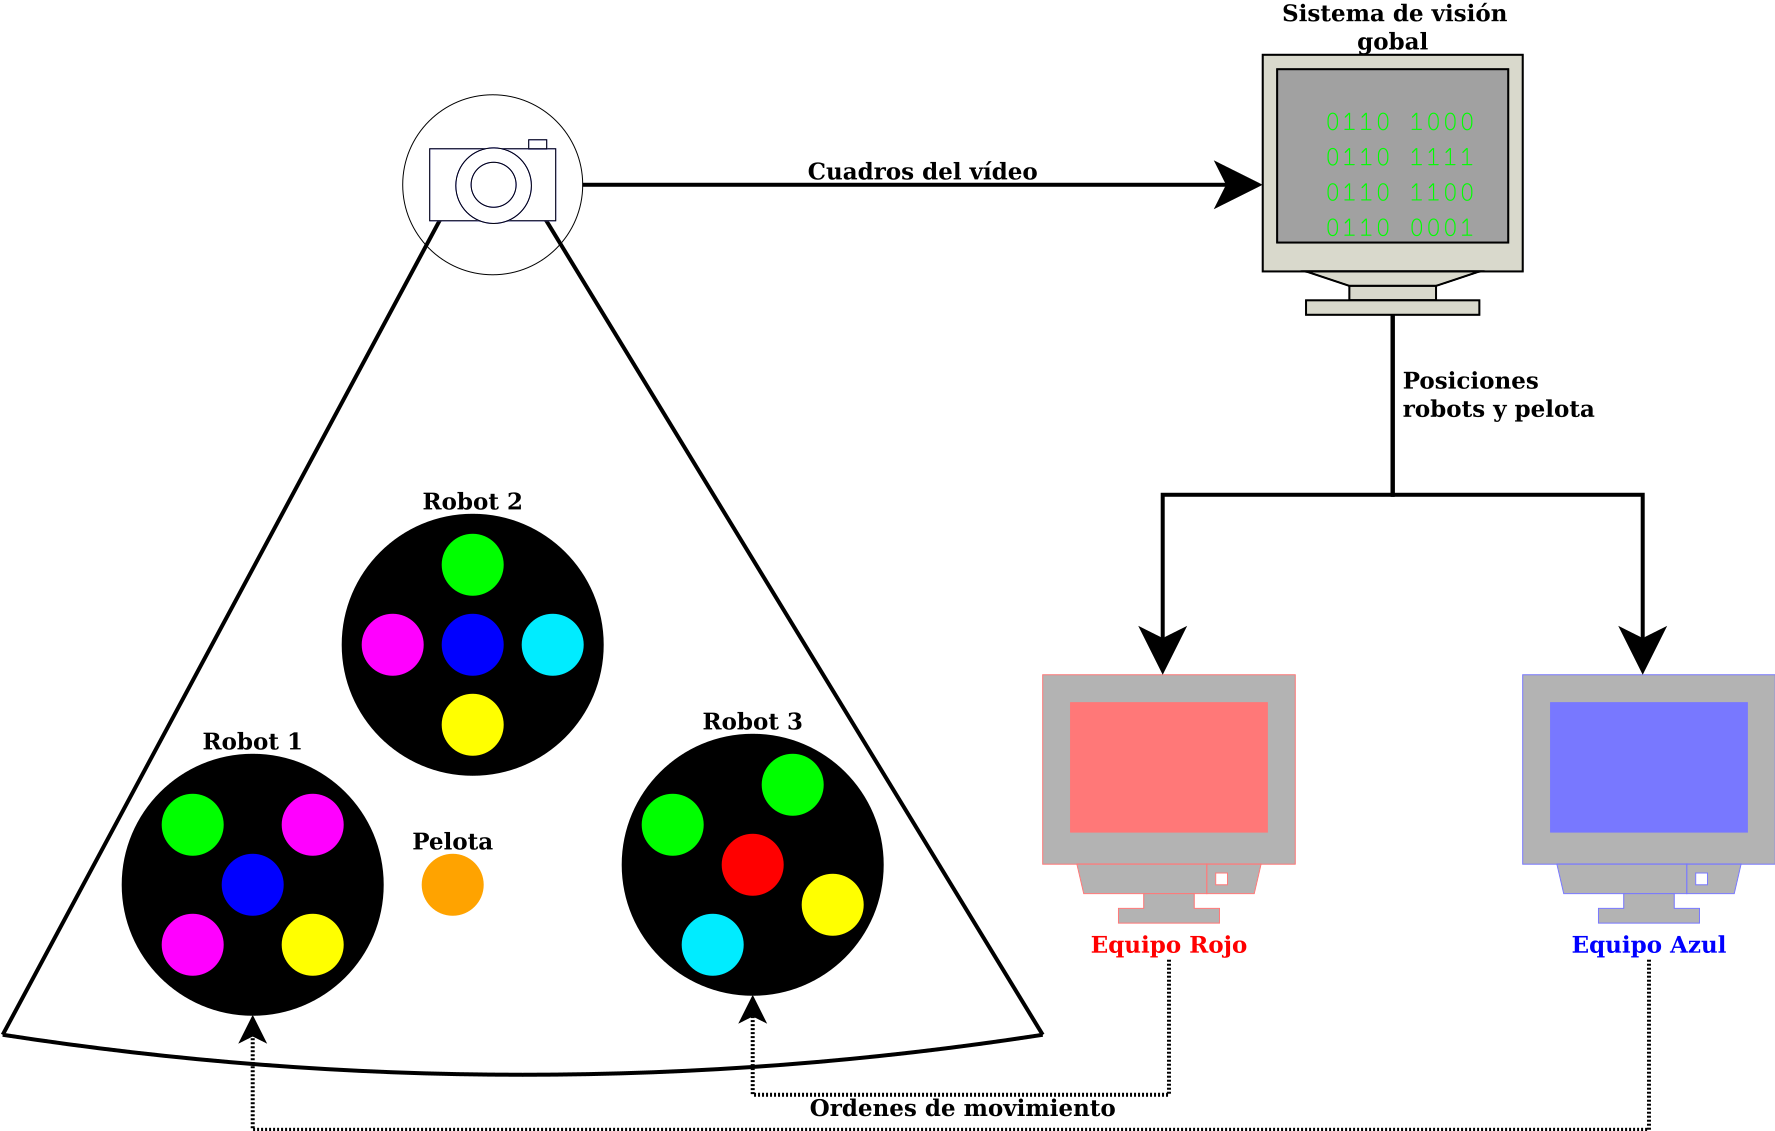
\includegraphics[width=\textwidth]{img/sistemaVG.pdf}
	\caption{Estructura de comunicación del sistema de visión global en
	fútbol de robots de la \emph{SSL}.}
	\label{sistemaVG}

\end{figure}

El uso de este sistema centralizado permite a los participantes abstraerse de
los problemas de la visión por computadora y enfocarse en la estrategia del
juego. Además, permite que las tareas de calibración y montaje de las cámaras se
realicen una sola vez para cada campo de juego en vez de para cada partido.

Originalmente el tamaño de la cancha era de 4,9$m$x3,4$m$, lo que permitía que
todo el campo de juego fuera observado con una sola cámara. Luego se opto por
dos tipos de canchas en los partidos de la \emph{SSL}: las canchas de tamaño
simple, con un tamaño de 6,05$m$x4,05$m$ para las cuales se utilizan dos
cámaras, una sobre cada media cancha, y las de tamaño doble, con un tamaño de
8,09$m$x6,05$m$, que utilizan cuatro cámaras, una por cada mitad de cada media
cancha. Desde el 2015 las canchas de tamaño doble son las utilizadas de forma
predeterminada\cite{sslrules2015}. Con este cambio se espera permitir la
exploración de nuevas tácticas por parte de los equipos, ya que mayor área
permite mayor movilidad. Sin embargo, esto trae aparejado el problema de que en
las canchas de tamaño doble se debe procesar cuatro veces la información que en
las canchas originales.

Aunque las reglas de la \emph{SSL} no establecen una resolución o taza de
cuadros para los vídeos capturados por las cámaras, en \cite{torres2014} se
comprobó que para una cancha de tamaño simple, un vídeo con una resolución de
352x288 píxeles, es suficiente para encontrar los robots y pelota en el $99\%$
de los cuadros. Por lo tanto, un vídeo de 800x600 píxeles es suficiente para la
totalidad de una cancha de tamaño doble.


% vim: set spell spelllang=es syntax=tex :

\section{Algoritmos paralelos y visión por computadora}

\label{algoritmosParalelosYVision}

En la actualidad la mayoría de los equipos de escritorio tienen más de un solo
núcleo de procesamiento. Según la encuesta de hardware de la plataforma de
distribución digital \emph{Steam} de marzo del 2017 \cite{steamSurvey}, solo
el $1.93$\% de los equipos donde esta instalado posee un solo núcleo. Esto se
ve acompañado de la capacidad actual de las placas aceleradoras de vídeo de
realizar procesamiento de propósito general permitiendo el procesamiento
masivamente paralelo en una computadora personal de gama media. Esta tendencia
se extiende también a otros equipos de computación como computadoras
portátiles, celulares y consolas de vídeo juegos, ya sean portátiles o no.

Reconociendo la importancia del desarrollo de aplicaciones paralelas, la Red
de Universidades Nacionales con Carreras Informáticas (\emph{RedUNCI}) incluye
en la lista de descriptores curriculares \emph{Algoritmos secuenciales,
concurrentes, distribuidos y paralelos}, \emph{Concurrencia y paralelismo}, y
\emph{Arquitecturas multiprocesador} \cite{RedUNCI2015}. El interés en estos
descriptores se ve reflejado en el hecho de que se recomiendan para las
carreras de grado Licenciatura en Ciencias de la Computación, Licenciatura en
Sistemas de Información, y Licenciatura en Informática. Las dos primeras son
dictadas actualmente en la facultad de informática de la \texttt{Universidad
Nacional del Comahue}, mientras que la tercera se encuentra en proceso de
diseño.

Dado el gran volumen de datos que deben manejar y su tendencia a la localidad
espacial, los sistemas de visión por computadora se ven muy beneficiados por
las capacidades de paralelismo del hardware actual. En 2004 se propuso por
primera vez un algoritmo implementando una red neuronal artificial de dos
capas ejecutando en una placa aceleradora de vídeo \cite{GPUforMLA}. Desde ese
entonces el uso de placas aceleradoras de vídeo han demostrado su utilidad en la
ejecución de redes neuronales de convolución. Este tipo especifico de redes
neuronales artificiales, cuyo funcionamiento esta basado en el cortex visual,
son especialmente útiles para resolver problemas de visión por computadora. Su
capacidad de reconocimiento y su velocidad de respuesta cuando se ejecutan en
sistemas masivamente paralelos permiten ser utilizadas incluso para el control
de vehículos autónomos \cite{e2eLearning4SDC}.

Ademas del incremento de las capacidades de procesamiento se a visto un
incremento en la capacidad de captura de información, dispositivos como cámaras
y acelerómetros son cada ves más baratos y pequeños. Dado que los sensores
pueden están montados sobre dispositivos con reducido poder de procesamiento,
normalmente los datos son enviados a ``la nube'', lo cual puede ser problemático
por los limites de ancho de banda y las dudas de la privacidad de los datos.
Para el caso particular donde el procesamiento se realiza a través de redes
neuronales de convolución, en \cite{pipelinebasedCaffe2017} se propuso un
esquema que permite atenuar ambos problemas. El esquema consiste en dividir la
red neuronal en dos partes, las primeras $N$ capas son ejecutadas en el
dispositivo donde están montados los sensores, y el resto de las capas son
ejecutadas en un servidor remoto. El éxito de este trabajo plantea la
posibilidad de dividir en trabajo en más capas, ejecutando capas intermedias en
una computadora del usuario dentro de la red local con el fin de enviar al
servidor externo menor cantidad de datos e información sensible.

Por estos motivos es deseable que los alumnos de las asignaturas de visión por
computadora puedan incorporar conceptos de computación paralela.


% vim: set spell spelllang=es syntax=tex :

\section{Sistemas existentes de visión global para fútbol de robots físicos}

\label{svgExistentes}

El software de visión global utilizado en la \emph{SSL} de la \emph{RoboCup} es
el \emph{SSL-Vision} \cite{sslvision}. Este es un sistema programado en
\emph{C++} basado en plugins, lo que le permite ser extendido fácilmente.
Lamentablemente, posee algunas desventajas con relación a la escalabilidad y al
uso educativo.

\begin{itemize}

	\item 	En primer lugar, el sistema de captura de cuadros y el de
		procesamiento están fuertemente acoplados, formando parte del
		mismo hilo de ejecución. Esto impide hacer uso de este sistema
		con el fin de incorporar la temática de procesamiento paralelo
		en el procesamiento de imágenes. Además limita su escalabilidad,
		ya que sin importar el sistema en el cual sea utilizado, nunca
		utilizará más de dos unidades de procesamiento (una para el hilo
		de ejecución de interfaz de usuario y otra para el hilo de
		ejecución para la captura y procesamiento).

	\item 	En segundo lugar, para aumentar la eficiencia del sistema, los
		plugins están altamente optimizados, aumentando la complejidad
		del sistema. Esta complejidad dificulta su uso como herramienta
		didáctica para la introducción al tema de la visión por
		computadora.

\end{itemize}

Abordando estos problemas, en \cite{torres2014} se presenta un sistema destinado
al uso educativo, basado en pilas de plugins, y también programado en
\emph{C++}. El sistema está planteado como un framework de construcción de
aplicaciones que permite elaborar diferentes estrategias y medir su rendimiento,
sin necesidad de construir una aplicación desde cero para cada una de ellas. En
el trabajo citado se ha validado el framework mediante la construcción y prueba
de una instancia de aplicación de servidor de video para un campeonato de fútbol
de robots reales.

La capacidad de respuesta a las restricciones de tiempo real del servidor así
construido fueron probadas en condiciones acordes a las presentadas en las
competencias. Se estableció un tiempo máximo de procesamiento de cuadro
admisible. Se midió el porcentaje de cuadros para los cuales el tiempo de
procesamiento superaba este máximo, hallando que este porcentaje quedaba dentro
de los objetivos de tolerancia.

La programación del framework propone un enfoque multi-hilo con el propósito de
mejorar la escalabilidad en microprocesadores multi-core. Utiliza dos hilos de
búsqueda de objetos: uno para encontrar la pelota y otro para encontrar los
robots; un hilo de captura de cuadros de video (desde un video grabado
previamente o una captura desde una cámara), y finalmente otro para la interfaz
de usuario. Su grado de paralelismo es mejor que el de \emph{SSL-Vision}; pero
aún así, al organizar el cómputo en tan sólo cuatro hilos en total, su diseño
está acoplado a una arquitectura de, a lo sumo, cuatro núcleos. Por lo tanto, no
resulta capaz de aprovechar plenamente las capacidades de plataformas de
hardware con mayores recursos.

Bajo las condiciones para las que fue diseñado este framework, el
desaprovechamiento de los recursos de hardware no es un problema, ya que, sobre
el hardware utilizado para las pruebas, el sistema puede procesar un video de
352$\times$228 píxeles a una tasa de 60 cuadros por segundo. Sin embargo, en las
competencias actuales se utilizan cuatro cámaras como origen de los datos de
video, en lugar de la cámara única para la cual el sistema fue diseñado.

Como punto de partida de la presente tesis, nos formulamos la pregunta de si el
framework soportaría este nuevo caudal de información. En este caso, si cada
cámara captura un video con una resolución de 352$\times$228, en una cancha de
tamaño simple el video compuesto resultante tendrá una resolución levemente
inferior a 800$\times$600 píxeles.  Al probar el servidor de video, construido
sobre el framework, con un video de esa resolución el número de cuadros por
segundo procesados cayó a 45 cuadros por segundo.

Esta diferencia en prestaciones muestra que la utilidad del sistema se ve
comprometida a medida que el volumen de los datos aumenta. Como las cuatro
cámaras de las competencias actuales pueden ofrecer una carga agregada todavía
superior a la utilizada en el experimento, resulta de interés abordar una mejora
de escalabilidad en la arquitectura de software del framework, a fin de
permitirle hacer frente a los cambios de escala en el problema.


% vim: set spell spelllang=es syntax=tex :

\section{Objetivos}

En \cite{torres2014}, se comprobó que para media cancha de una cancha de tamaño
simple es suficiente trabajar con un vídeo con una resolución de 352x288
píxeles. Por ende, para poder capturar una cancha de tamaño completo se necesita
un vídeo con una resolución de al menos 704x576 píxeles. Por lo tanto, el
principal objetivo de este trabajo sera el diseño e implementación de un sistema
de visión global paralelo capaz de procesar un vídeo de 800x600 píxeles de
resolución a 60 cuadros por segundo y que sea capaz aprovechar paralelismo que
provee el hardware actual.

El objetivo secundario es que el sistema desarrollado sea de fácil modificación
y adaptación. Para lograr esto, se definirá en principio un framework y sobre
este se construirá una solución especifica para el fútbol de robots.


% vim: set spell spelllang=es syntax=tex :

\section{Metodología}

Para comprobar la adaptabilidad del software desarrollado por Guillermo Torres
se grabo un nuevo vídeo. De este se crearon tres versiones con distintas
resoluciones, 1280x720 píxeles, 800x600 píxeles, 352x224 píxeles, cada uno con
una taza de 60 cuadros por segundo. Se realizaron corridas con cada uno de estos
vídeos en una computadora con un procesador Intel Xeon E5-2630. Este es un
procesador de 12 núcleos y con un reloj de 2,30GHz. El equipo cuenta ademas con
16GiB de memoria ram.

Durante la prueba con el vídeo de resolución 352x224 el sistema pudo procesar
todos los cuadros del vídeo a tiempo (60 cuadros por segundo). Esto era de
esperarse, ya que el sistema fue pensado con tal resolución en mente. Sin
embargo a pesar de la velocidad y cantidad de los núcleos, con el vídeo de
resolución 800x600 píxeles la cantidad de cuadros por segundo cayo a 45. Para el
vídeo de resolución 1280x720, la reducción del rendimiento fue mas brusca,
decayendo a 14 cuadros por segundo.

Para resolver este problema se pueden aplicar tres enfoques distintos:

\begin{itemize}

\item	Se pude resolver el problema optimizando cada uno de los \emph{plugins}
	del framework, esperando de esta manera que el tiempo de procesamiento
	de cada cuadro se reduzca lo suficiente como para que el sistema pueda
	procesar la mayoría de los cuadros a tiempo.

\item	Se puede hacer provecho de que los mecanismos para obtener la
	información de los cuadros no mantienen información entre ellos (es
	decir, para el sistema los cuadros son independientes). Dada la
	disponibilidad de recursos, se pueden procesar múltiples cuadros al
	mismo tiempo sin que esto genere diferencias en la información obtenida
	(salvo por el orden). Esto permitiría aumentar la cantidad de cuadros
	por segundo obtenidos, aunque el tiempo de procesamiento de cada uno se
	mantenga igual.

\item	Para realizar la búsqueda de los objetos, el cuadro puede ser dividido.
	Esto permitirá realizar la búsqueda en cada zona en paralelo. Para el
	correcto funcionamiento, las zonas deberán tener partes en común que
	dependerán del tamaño de los objetos, ya que no debe suceder que un
	objeto no aparezca completo en ninguna de las zonas. Esto permitiría
	reducir el tiempo de procesamiento de cada cuadro.

\end{itemize}

Lamentablemente el primer enfoque es muy especifico de la solución para ser
aplicada en el \emph{framework}. Ademas no fomenta la experimentación, ya que
cada \emph{plugin} que se agregue o modifique deberá ser optimizado. El segundo
y tercer enfoque son suficientemente generales como para ser aplicados como
parte del \emph{framework}, permite agregar y modificar los \emph{plugins} sin
mayores dificultades, y en el caso en el cual una solución especifica no cumpla
con las condiciones que permitan aplicar alguna de las soluciones se puede
limitar el paralelismo (ya sea no dividiendo el cuadro o procesando solo uno por
vez).


% vim: set spell spelllang=es syntax=tex :

\section{Organización del trabajo}

El resto del trabajo continuará con el capítulo \ref{marcoTeorico} donde se
presenta el marco teórico necesario para este trabajo. La sección
\ref{mt_visionComputadora} es una introducción a la visión por computadora y las
etapas que suelen definirse en un sistema de visión por computadora. En la
sección \ref{descripcionSistemaBase} se detalla el sistema de visión global
utilizado como base para el desarrollo del sistema propuesto en este trabajo.
En la sección \ref{mt_openmp} se hace una introducción a \emph{OpenMP} y se
explican sus modelos de computación y las directivas utilizadas por el sistema
propuesto.

En el capítulo \ref{sistemaPropuesto} se describe el sistema propuesto. La
sección \ref{descripcionSistema} describe las tareas del sistema y la forma en
la cual se fragmentan los datos. Luego, en la sección
\ref{implementacionFramework}, se describe la implementación.

En el capitulo \ref{experimentacion} se describen los experimentos realizados
utilizando el sistema desarrollado. Se comienza explicando la metodología
experimental en la sección \ref{metodologiaExperimental}, la plataforma
experimental se detalla en la sección \ref{plataformaExperimental}, y los
detalles de los experimentos y sus resultados son discutidos en la sección
\ref{resultados}.

En el capítulo \ref{usoEducativo} se plantean posibles usos del sistema como
herramienta didáctica para materias de sistemas paralelos y visión por
computadora.

Finalmente en el capitulo \ref{conclucionesYTrabajosFuturos} se presentan las
conclusiones del trabajo, en la sección \ref{concluciones}, y los posibles
trabajos futuros, en la sección \ref{trabajosFuturos}.


\chapter{Marco teórico}

\label{marcoTeorico}

% vim: set spell spelllang=es syntax=tex :

\section{Visión por computadora}

La visión por computadora es una disciplina cuyo objetivo principal es definir
un modelo de una escena a partir de imágenes\cite{cvLinda2001}, en el caso del
fútbol de robots, el modelo que se quiere definir es la posición de los robots y
la pelota dentro de la cancha. La disciplina engloba el estudio de métodos
captura, mejoramiento, y extracción de información. Dependiendo de la
aplicación, existen distintas etapas para la obtención de la información y su
procesamiento, pero por lo general se definen los siguientes
pasos\cite{digitalImageProcessing2ed,wikiCV}:

\begin{description}

	\item[Adquisición de la imagen:] Se trata de la digitalización de la
		imagen a procesar. Esta puede ser obtenida de uno o mas
		sensores. Distintos sensores pueden capturar distintas bandas
		del espectro electromagnético. El resultado puede variar desde
		una imagen bidimensional monocromática hasta volúmenes
		tridimensionales.
	
		En el fútbol de robots de tamaño pequeño, el conjunto de cámaras
		capturan serie de imágenes bidimensionales a color. El sistemas
		de coordenadas de la imagen es normalmente \emph{RGB} o
		\emph{YUV}.

	\item[Pre procesamiento:] Para que la imagen pueda ser procesada, muchas
		veces es necesario aplicarle transformaciones que no extraen
		información, pero son pre condiciones para las siguientes etapas
		de procesamiento. Algunas de las transformaciones comunes son
		corrección de color, reducción de ruido o cambio de espacio de
		color.

		Los sistemas de visión global para el fútbol de robots de la
		\emph{SSL} suelen trabajar con el espacio de color \emph{YUV},
		por lo que de ser necesario, la imagen debe ser convertida a
		este espacio de color. Otro pre procesamiento que puede
		realizarse es componer las imágenes del conjunto de cámaras en
		una sola imagen.

	\item[Extracción de características:] Consiste en el reconocimiento de
		características de bajo nivel como puntos de interés, bordes,
		regiones y masas. Los sistemas para la \emph{SSL} suelen en esta
		etapa reconocer las masas de colores de los parches y la pelota.

	\item[Detección y Segmentación:] Se trata de separar la imagen en sus
		partes constituyentes y seleccionar aquellas de interés. Los
		sistemas de visión global para fútbol de robots de la \emph{SSL}
		utilizan las masas de color reconocidas en la etapa anterior
		para encontrar los robots y la pelota.

	\item[Procesamiento de alto nivel:] En esta etapa se crea finalmente el
		modelo de la escena utilizando los resultados de las etapas
		anteriores. En fútbol de robots de la \emph{SSL} se toman las
		posiciones dentro de la imagen de los robots y pelota
		encontrados en la etapa anterior y se calcula su posición dentro
		de la cancha de acuerdo con la geometría de esta.

	\item[Toma de decisiones:] Muchas de las aplicaciones de visión por
		computadora integran la toma de decisiones como parte del
		proceso, en lugar de solo informar. En el caso de los sistemas
		de visión global para fútbol de robots, el sistema solo notifica
		a las computadoras de los equipos la posición de los robots y
		pelota.

\end{description}


% vim: set spell spelllang=es syntax=tex :

\section{Descripción del sistema de visión global para fútbol de robots físicos
sobre el que se basa la presente propuesta}

\sectionmark{Descripción del sistema de visión global para fútbol de robots...}

\label{descripcionSistemaBase}

El principal objetivo del sistema descripto en \cite{torres2014} es su
utilización como herramienta didáctica para la introducción a la visión por
computadora. El sistema define un framework de visión por computadora capaz de
adaptarse a distintos dominios, pero en el trabajo se ofrece una solución
específica para el fútbol de robots de la liga de tamaño pequeño.

El sistema está basado en pilas de plugins y utiliza múltiples hilos para
aprovechar hasta cuatro núcleos (para el fútbol de robots); pero si la
plataforma posee más núcleos, no serán utilizados. Cada uno de los hilos tiene
una responsabilidad diferente. El framework general tiene tres componentes
principales:

\begin{description}

	\item[Hilo principal:] es el hilo encargado de la interfaz gráfica de
		usuario.

	\item[Hilo de captura de cuadros:] es el hilo encargado de la captura o
		generación de los cuadros a partir de una cámara o archivo. El
		hilo de captura está desacoplado de los hilos de búsqueda o
		procesamiento de cuadros.

	\item[Hilos de procesamiento de cuadros:] estos hilos están formados por
		una pila de plugins que procesarán cada cuadro en forma
		secuencial. Normalmente, por cada tipo de objeto a reconocer,
		hay un hilo de este tipo dedicado a su detección. La diferencia
		entre ellos está en los plugins que componen la pila y en su
		orden. Existen mecanismos de control para asegurar que, si un
		cuadro es procesado por un hilo de procesamiento, entonces
		también será procesado por el resto de los hilos de
		procesamiento, asegurando al mismo tiempo que cada cuadro será
		procesado sólo una vez por cada hilo.

\end{description}

En la implementación de la solución específica para el fútbol de robots de la
\emph{SSL}, se crean dos hilos de procesamiento de cuadros, uno para la búsqueda
de los robots y el otro para la búsqueda de la pelota. Las primeras etapas de
procesamiento son iguales en ambos. Los primeros plugins son los de
\emph{conversión de color}, \emph{segmentación de color} y \emph{morfología}. El
hilo de procesamiento que busca la pelota continúa con el plugin de
\emph{búsqueda de pelota}, mientras que aquél encargado de la búsqueda de robots
continúa con los plugins de \emph{detección de regiones principales} y
\emph{detección de regiones secundarias}. Ambos terminan con el plugin de
\emph{difusión}. En la figura \ref{pilasPlugins} se muestran ambas pilas y los
plugins que las componen. Como ambas pilas ejecutan los primeros tres plugins
sobre el mismo cuadro, se plantea la posibilidad de ejecutarlos una sola vez por
cuadro.

\begin{figure}[!htb]

	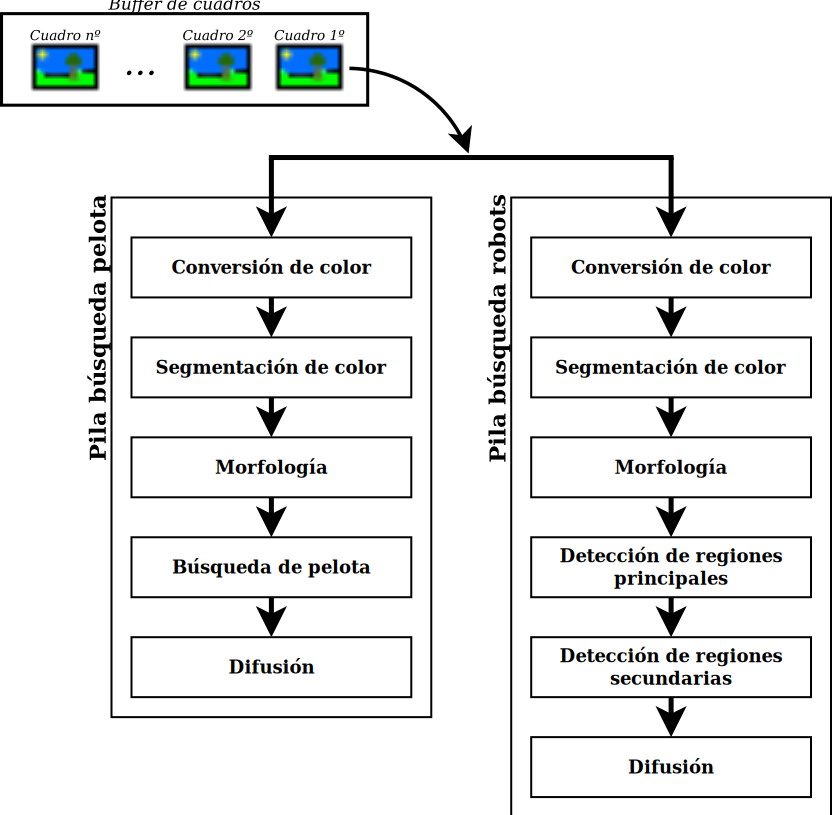
\includegraphics[width=\textwidth]{img/pilas.pdf}

	\caption{Pilas de plugins del sistema propuesto en \cite{torres2014}.}

	\label{pilasPlugins}

\end{figure}


De acuerdo a su función, los plugins pueden ser agrupados por las etapas de la
visión por computadora que implementan:

\begin{description}

	\item[Adquisición de la imagen:] Esta etapa está a cargo del hilo de
		captura de cuadros.

	\item[Preprocesamiento:] plugins de conversión de color, de segmentación
		de color y de morfología.

	\item[Extracción de características, Detección y Segmentación:] plugins
		de detección de regiones principales.

	\item[Procesamiento de alto nivel:] plugins de detección de pelota y de
		detección de regiones secundarias.

	\item[Toma de decisiones:] Dado que el sistema de visión para fútbol de
		robots no realiza toma de decisiones, el estado de la cancha es
		comunicado a las computadoras de los equipos a través del plugin
		de difusión.

\end{description}

El tiempo de generación de cuadros es fijo (o a demanda), mientras que el de
procesamiento es variable, pudiendo ser mayor o menor que el tiempo de
generación. Por ello, cuando se genera un nuevo cuadro, éste se coloca en un
buffer. Si la capacidad de procesamiento es insuficiente, y no hay más espacio
en el buffer para almacenar un nuevo cuadro, se descarta el cuadro más viejo.
Esta estrategia da mayor prioridad a la información más actual.



% vim: set spell spelllang=es syntax=tex :

\section{OpenMP: Open Multi-Processing}

\label{mt_openmp}

\emph{OpenMP} es una API de bibliotecas y directivas al compilador para la
definición de paralelismo de alto nivel para sistemas \emph{MIMD} de memoria
compartida en \emph{C}, \emph{C++} y \emph{Fortran} \cite{ompWeb}. Es una API
abierta, publicada y definida por el consorcio \emph{OpenMP Architecture Review
Board} (o \emph{OpenMP ARB}). El consorcio está compuesto por representantes de
las industrias del hardware y software. Sus miembros permanentes son \emph{AMD},
\emph{ARM}, \emph{CRAY}, \emph{Fujitsu}, \emph{HPE}, \emph{IBM}, \emph{Intel},
\emph{Micron}, \emph{NEC}, \emph{NVIDIA}, \emph{Oracle}, \emph{Red Hat}, y
\emph{Texas Instruments} y, sus miembros temporales incluyen al centro de
cómputo Barcelona, la \emph{NASA} y \emph{cOMPunity}, entre otros \cite{ompWeb}.
La primera publicación de \emph{OpenMP} fue su versión para \emph{Fortran} en
octubre de 1997, las especificaciones para \emph{C} y \emph{C++} fueron
publicadas en octubre de 1998.

\emph{OpenMP} permite la creación de regiones paralelas, secciones críticas,
tareas y puntos de sincronización, simplemente marcando un bloque de código
con unas pocas directivas al compilador. Originalmente implementaba sólo el
modelo de \emph{fork and join}, pero a partir de la versión 3.0 se agregó el
modelo de tareas explícitas \cite{openmp08}. Ambos modelos fueron utilizados
para la implementación del sistema.

El modelo de \emph{fork and join} fue propuesto por primera vez en
\cite{conway1963}. En este modelo, la ejecución del programa está a cargo de un
solo hilo al comienzo de la ejecución y durante sus secciones secuenciales. El
hilo inicial es llamado hilo principal. Cuando se encuentra una región de
trabajo compartido (o \emph{worksharing region}) de $N$ tareas, el hilo
principal crea $N-1$ nuevos hilos. Cada hilo (incluido el hilo principal)
ejecuta una de las $N$ tareas. Esta etapa es llamada \emph{fork}. El hilo
principal no continúa la ejecución secuencial hasta que no han finalizado todas
las tareas paralelas. A esta sincronización se la llama \emph{join}. La figura
\ref{conway} muestra un ejemplo en el cual se crean dos tareas paralelas.
\emph{OpenMP} extiende el modelo permitiendo que la cantidad de hilos sea menor
que la cantidad de tareas, cuando esto sucede, las tareas sin hilo asignado son
colocadas en una lista de tareas en espera. Cuando un hilo termina de ejecutar
una tarea, si hay tareas esperando en la lista de tareas en espera, toma una y
la ejecuta. El modelo de \emph{fork and join} puede aplicarse tanto para
paralelismo de tareas como de datos.

\begin{figure}[!htb]

	\centering

	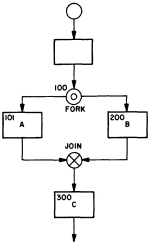
\includegraphics[height=0.25\textheight]{img/conway.pdf}

	\caption{Descripción original del modelo de \emph{fork and join}
	presentado por Melvin Conway en 1963 \cite{conway1963}.}

	\label{conway}

\end{figure}

Dado que la creación de hilos suele ser una operación costosa, la mayoría de las
implementaciones de \emph{OpenMP} suelen no destruir los hilos creados durante
el \emph{fork}, si no que se mantienen inactivos para ser reutilizados cuando se
encuentre otra región de trabajo compartido.

El segundo modelo implementado en \emph{OpenMP} a partir de la versión 3.0 es el
de tareas. Este modelo permite la creación de nuevas tareas explícitas dentro de
una región de trabajo compartido. Cuando se encuentra un área de trabajo
compartido, se crean una o más tareas implícitas y $N$ hilos de ejecución. Al
igual que el modelo de \emph{fork and join} extendido, la cantidad de hilos
puede ser menor que la cantidad de tareas, pero también puede ser mayor. Durante
la ejecución una tarea, ésta puede crear nuevas tareas explícitas a través de la
directiva \emph{task}. Si hay hilos de ejecución libres, la nueva tarea será
asignada a uno de ellos, sino es colocada en una lista de tareas en espera.
Cuando un hilo termina de ejecutar una tarea, toma otra de la lista de tareas en
espera de tareas o espera. Sólo se destruyen los hilos al terminar la ejecución
de todas las tareas y salir de la región de trabajo compartido.

\subsubsection{Directivas de OpenMP}

El control de la creación de hilos y tareas en \emph{OpenMP} se realiza a través
de directivas al compilador. En esta sección mencionaremos aquellas utilizadas
por el sistema propuesto. En \emph{C} y \emph{C++} todas las directivas toman la
forma de \textbf{\#pragma omp DIRECTIVA [OPCIONES]}.

\begin{itemize}

	\item	La directiva más utilizada es \emph{parallel [num\_threads(N)]},
		ésta define una región de trabajo paralelo y crea $N-1$ hilos de
		ejecución (si no se incluye \emph{num\_threads(N)}, la cantidad
		de hilos se establece por medio de una variable global, y en
		caso de que ésta no esté definida, dependerá de la
		implementación). Cada hilo ejecutará una tarea definida por el
		bloque inmediato a la directiva, implementando el modelo
		\emph{fork and join}.

	\item	Si se desea que un bloque sea ejecutado sólo por un hilo se pueden
		utilizar las directivas \emph{single} y \emph{master}. Éstas
		asegurarán que el bloque inmediato sea ejecutado sólo por uno de
		los hilos del grupo. En el caso de la directiva \emph{single},
		cualquiera de los hilos del grupo podrá ser elegido para
		ejecutar el bloque, mientras que en el caso de \emph{master},
		sólo el hilo principal del grupo lo ejecutará.

	\item	Para la creación de una región de trabajo compartido bajo el
		modelo de tareas, se utiliza la directiva \emph{parallel
		num\_threads(N)} para crear los $N$ hilos de ejecución, seguida
		de la directiva \emph{master} o \emph{single} para que sólo el
		hilo principal ejecute la tarea que crea las primeras tareas de
		la región de trabajo compartido.
	
	\item	Para la creación de cada tarea se debe utilizar la directiva
		\emph{task} seguida del bloque que contiene el código a ejecutar
		por la tarea.

	\item	Si un hilo necesita esperar la finalización de las tareas que
		creó, antes de continuar su ejecución, puede utilizar la
		directiva \emph{taskwait}.

	\item	Si se desea que cada hilo ejecute una tarea con código distinto se
		debe utilizar la directiva \emph{parallel sections
		num\_threads(N)}. El bloque inmediato debe contener a su vez
		bloques precedidos por la directiva \emph{section}. Al igual que
		\emph{parallel}, esta directiva define una región de trabajo
		paralelo de $N$ hilos, pero el código de cada tarea está
		definido por los bloques inmediatos a las directivas
		\emph{section}. En caso de que se creen más hilos que las tareas
		definidas, los hilos sobrantes no ejecutarán. El modelo
		implementado por esta directiva es \emph{fork and join}.

	\item	Para definir secciones críticas se pueden utilizar las directivas
		\emph{critical [NOMBRE]} y \emph{atomic}. La primera permite
		definir un bloque de complejidad arbitraria como sección
		crítica, e incluso permite definir bloques distintos como la
		misma sección crítica si comparten el mismo nombre. La segunda
		directiva sólo acepta bloques en los cuales se realiza una
		operación aritmética simple, y resulta en una implementación
		más eficiente.

\end{itemize}

En la figura \ref{directivas} se muestra un código de ejemplo del uso de las
directivas presentadas junto con un diagrama mostrando una posible secuencia
de ejecución.

\begin{figure}[!htb]

	\centering

	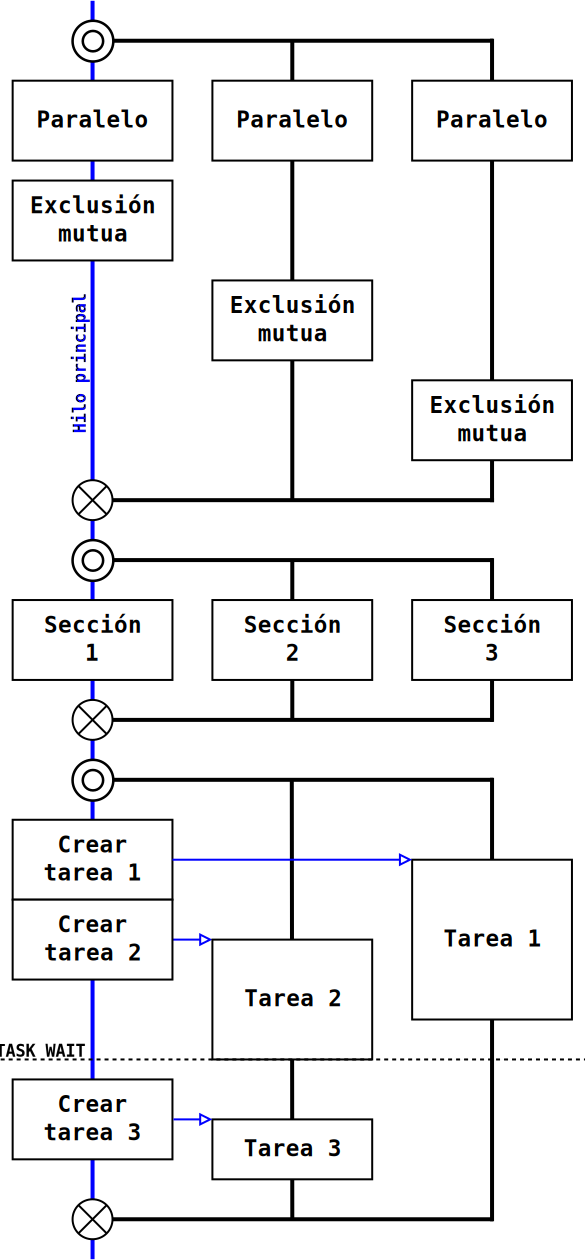
\includegraphics[height=0.40\textheight]{img/directivasOMP.pdf}
	\includegraphics{img/codigoDirectivasOMP.pdf}

	\caption{Código de ejemplo de uso de directivas de \emph{OpenMP} y
	posible secuencia de ejecución.}

	\label{directivas}

\end{figure}


\chapter{Sistema propuesto}

\label{sistemaPropuesto}

% vim: set spell spelllang=es syntax=tex :

En este capitulo comenzaremos analizando las estrategias de paralelización
disponibles y justificaremos la selección de una de ellas. Esto nos permitirá
establecer las distintas tareas que ejecutara el framework y como se dividirán
los datos. Finalmente, una ves establecida la estructura del sistema, se
trataran los detalles de la implementación.

\label{descripcionSistema}

\section{Discusión de las estrategias de paralelización}

Para aumentar el throughput del sistema se pueden aplicar cuatro enfoques distintos:

\begin{itemize}

	\item	Dado que en un vídeo ya decodificado el procesamiento de cada
		cuadro es independiente del procesamiento de los demás, y dada
		la disponibilidad de recursos de computo, se pueden procesar
		múltiples cuadros al mismo tiempo sin que esto genere
		diferencias en la información obtenida (salvo por el orden).
		Esto permitiría aumentar la cantidad de cuadros por segundo
		obtenidos, aunque el tiempo de procesamiento de cada uno se
		mantenga igual.

	\item	Para realizar la búsqueda de los objetos, el cuadro puede ser
		dividido. Esto permitirá realizar la búsqueda en cada zona en
		paralelo. Para el correcto funcionamiento, las zonas deberán
		tener partes en común cuyos tamaños dependerán del tamaño de los
		objetos (en este caso, los robots), ya que no debe suceder que
		un objeto no aparezca completo en ninguna de las zonas. Esta
		estrategia busca reducir el tiempo de procesamiento por cuadro
		mediante el uso de múltiples unidades de procesamiento abocadas
		al mismo cuadro. Ademas esta estrategia podría sacar provecho de
		una mayor localidad espacial.

	\item	Ya que la búsqueda de cada tipo de objetos es independiente de
		la búsqueda de los demás tipos, se pueden realizar múltiples
		búsquedas en paralelo sobre el mismo cuadro por cada tipo de
		objeto.

	\item	Se puede resolver el problema optimizando cada uno de los
		plugins del framework, esperando de esta manera que el tiempo de
		procesamiento de cada cuadro se reduzca lo suficiente como para
		que el sistema pueda procesar la mayoría de los cuadros a
		tiempo.

\end{itemize}

Lamentablemente este último enfoque dificulta su uso como herramienta didáctica,
ya que cada plugin que se agregue o modifique deberá ser optimizado. El primer y
segundo enfoque permiten agregar y modificar los plugins sin mayores
dificultades, y en el caso en el cual un plugin no cumpla con las condiciones
que permitan aplicar alguno de los enfoques, se puede limitar el paralelismo ya
sea no dividiendo el cuadro o procesando solo uno por vez.

Si bien el tercer enfoque también permitiría agregar o modificar los plugins
fácilmente, en las pruebas que se realizaron se comprobó que realizar las
búsquedas por cada tipo de objeto en paralelo sobre cada fragmento tenia un
efecto adverso. Por este motivo, el tercer enfoque no fue aplicado sobre el
producto final, y no sera incluido en las explicaciones siguientes. Los detalles
de los resultados que llevaron a tomar esta decisión serán explayados más
adelante en la sección de resultados.

\section{Tareas del sistema}

El sistema ejecuta tareas estáticas y tareas dinámicas. Las tareas estáticas son
aquellas que permanecen en ejecución desde el inicio del programa hasta su
finalización. Las tareas dinámicas son creadas para procesar un cuadro o
fragmento específico y una vez que terminan de procesar el cuadro o fragmento
finalizan. Como las tareas dinámicas son aquellas que realizan el procesamiento
para la búsqueda de los objetos, a las llamamos ``tareas de búsqueda''.

Según su funcionalidad, las tareas son clasificadas en cuatro tipos:

\begin{description}

	\item[Generación de cuadros:] Es la tarea encargada de la generación o
		captura de los cuadros y colocarlos en la cola de cuadros a
		procesar. Esta es una tarea estática, y sólo hay una en el
		sistema.

	\item[Generación de tareas de fragmentación de cuadro:] Esta tarea crea
		una tarea de fragmentación de cuadro para cada cuadro en la
		cola. Solo toma un cuadro de la cola si hay hilos de ejecución
		para tareas de búsqueda libres. Ésta es una tarea estática, y
		solo hay una en el sistema.

	\item[Fragmentación de cuadro:] Cada tarea de este tipo divide su cuadro
		en una cantidad predefinida de fragmentos de igual (o similar)
		tamaño. Luego, por cada fragmento, se crea una tarea de
		procesamiento de fragmento. Estas son tareas de búsqueda, y
		puede haber múltiples en el sistema.

	\item[Procesamiento de fragmento:] Cada una de estas tareas toma su
		fragmento asociado y lo procesa utilizando cada una de las pilas
		de plugins. Estas son tareas de búsqueda, y puede haber
		múltiples en el sistema.

\end{description}

\begin{figure}[!h]

	\centering

	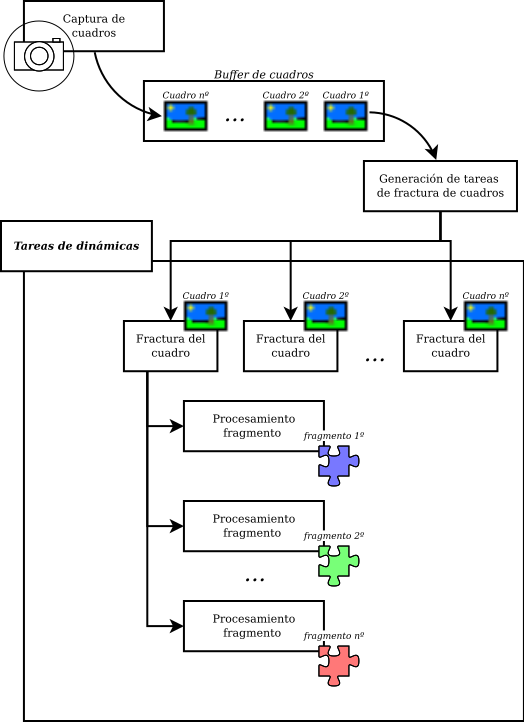
\includegraphics[height=0.45\textheight]{img/framework.pdf}

	\caption{Tareas principales del framework.}

	\label{tareasFramework}

\end{figure}

Cada una de las dos tareas estáticas tiene un hilo de ejecución asignado. Las
tareas de búsqueda son ejecutadas por un conjunto de $N$ hilos de
ejecución\footnote{$N$ es un parámetro de entrada del programa.}. Cuando un hilo
de ejecución (del conjunto) está libre, toma una nueva tarea de búsqueda para
ejecutar. Como estos hilos de ejecución son los que ejecutan las tareas de
búsqueda, nos referiremos a ellos como ``hilos de búsqueda''. En la figura
\ref{tareasFramework} se muestran un diagrama de las tareas del framework, y en
la figura \ref{hilosFramework} se muestra como las tareas son asignadas a los
hilos de ejecución.

La cantidad de hilos de ejecución del sistema es igual a la cantidad de hilos de
búsqueda más los dos hilos para tareas estáticas (generación de cuadros y
generación de tareas de fragmentación de cuadro). Por esto la cantidad de
unidades de procesamiento aprovechables esta principalmente determinado por la
cantidad de hilos de búsqueda.

\begin{figure}[!h]

	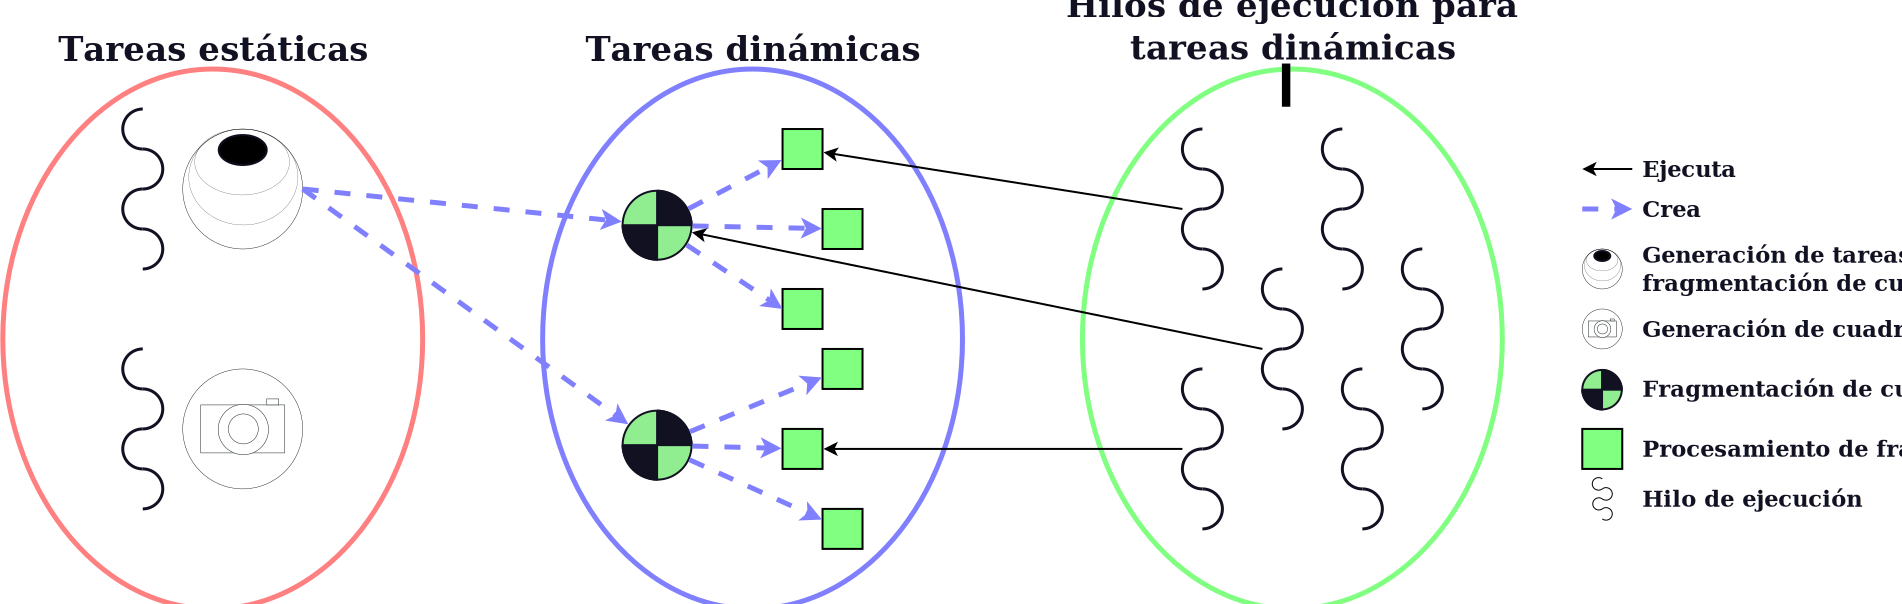
\includegraphics[width=\textwidth]{img/hilos.pdf}

	\caption{Asignación de tareas a los hilos de ejecución.}

	\label{hilosFramework}

\end{figure}

\section{Fragmentación del conjunto de datos}

Para poder realizar el procesamiento paralelo, el conjunto de datos debe ser
fragmentado, en el caso del framework propuesto la división se realizara en
dos niveles. Dado que el conjunto de datos es un vídeo, la primera
fragmentación consta de la separación en cuadros. Como cada cuadro es una
captura del ambiente completo en un instante de tiempo especifico distinto al de
los demás cuadros, se pueden procesar de forma independiente. La segunda
fragmentación de los datos se realiza dentro de cada cuadro. Ya que fragmentos
de un mismo cuadro contienen información distinta del ambiente sobre el mismo
instante, los fragmentos son dependientes entre si. Es por eso que se deben
tener consideraciones especiales para la división del cuadro.

Si el cuadro se divide en partes sin zonas solapadas puede suceder que los
parches de un robot se encuentren en fragmentos distintos. Esto es un problema,
ya que para encontrar los robots, el plugin de detección de robots debe detectar
todos los parches que lo identifican, por lo cual todos deben estar dentro del
mismo fragmento. Para asegurar esto, cada par de fragmentos adyacentes deben
compartir una zona igual al diámetro de un robot. En la figura
\ref{areaCompartida} se muestran los casos donde el área compartida es menor al
diámetro de un robot y donde el área compartida es del diámetro de un robot.

\begin{figure}[!h]

	\centering
	
\includegraphics[width=0.45\textwidth]{img/areaTooSmall.pdf}
	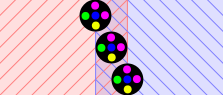
\includegraphics[width=0.45\textwidth]{img/areaPerfect.pdf}

	\caption{Izquierda: si el área compartida es demasiado pequeña y si el
	robot se encuentra entre dos fragmentos, puede que sus parches no sean
	completamente visibles desde ninguno de ellos. Derecha: si el área
	compartida es del ancho de los robots, entonces todos los parches son
	visibles completamente desde por lo menos un fragmento.}

	\label{areaCompartida}

\end{figure}

Dado que los fragmentos comparten una área en sus bordes, la suma del área de
los fragmentos es superior al área de la imagen original. Para reducir los
píxeles a procesar, se debe reducir la zona compartida. Como la zona compartida
tiene un ancho fijo (el diámetro de un robot), para encontrar el área compartida
mínima se debe minimizar el perímetro del fragmento.

Por la manera que las imágenes se representan comúnmente en una computadora y
por su simplicidad, se opto por trabajar con un teselado con rectángulos. En el
caso de estos, para minimizar su perímetro y maximizar su área, se debe procurar
que la relación entre su ancho y altura sea lo más cercana a uno. También, para
balancear la carga uniformemente, todos los fragmentos serán de igual tamaño.
El tiempo de procesamiento de un fragmento depende no solo de su área sino que
es influido por los elementos encontrados por los plugins, por lo cual
fragmentos de igual tamaño pueden tener tiempos de procesamiento muy distintos.
Sin embargo, dado que no poseemos más información antes del procesamiento,
consideramos que esta es la mejor heurística con la que contamos. Aquellos que
se encuentren en los bordes inferior y derecho pueden que sean más chicos.

En la figura \ref{fragmentos} se muestran como se divide un cuadro de 800x600
píxeles con un área compartida de 50 píxeles en 1, 2, 5 y 8 fragmentos. Cuando
el número de fragmentos es un número primo, como en el caso de 5 fragmentos, el
cuadro se divide en franjas de igual ancho o altura que el cuadro original. Este
tipo de división produce fragmentos con perímetros mayores, produciendo grandes
áreas compartidas.

\begin{figure}[!h]

	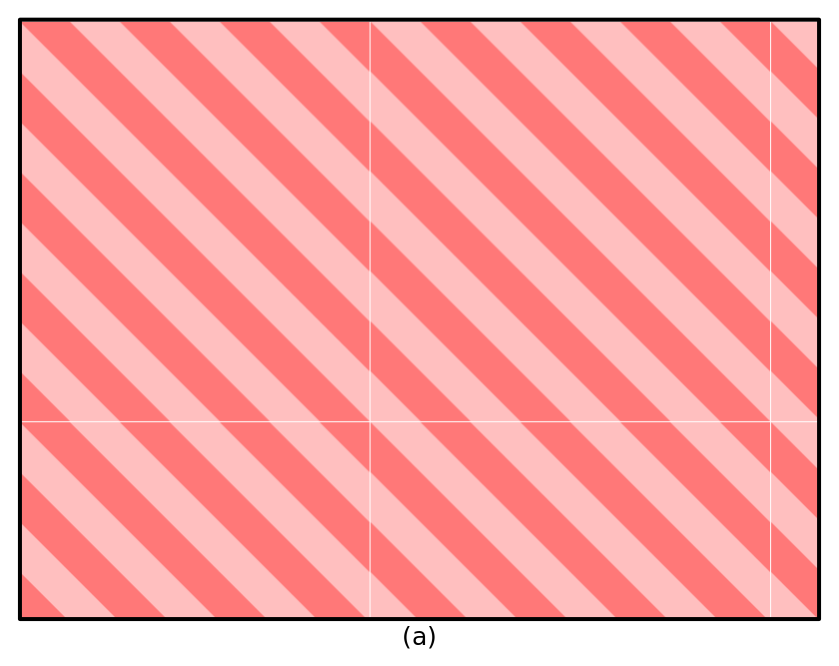
\includegraphics[width=0.5\textwidth]{img/fragmentos1.pdf}
	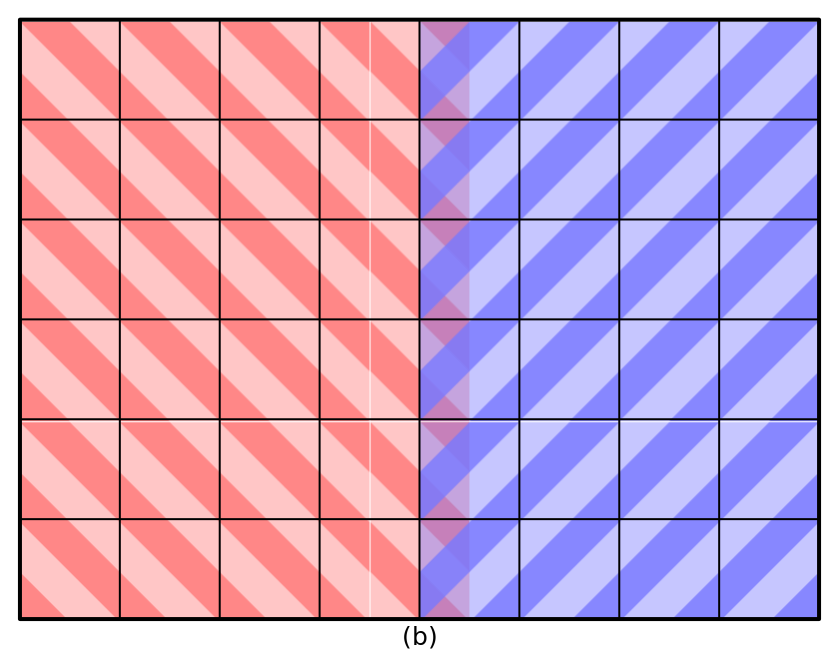
\includegraphics[width=0.5\textwidth]{img/fragmentos2.pdf}
	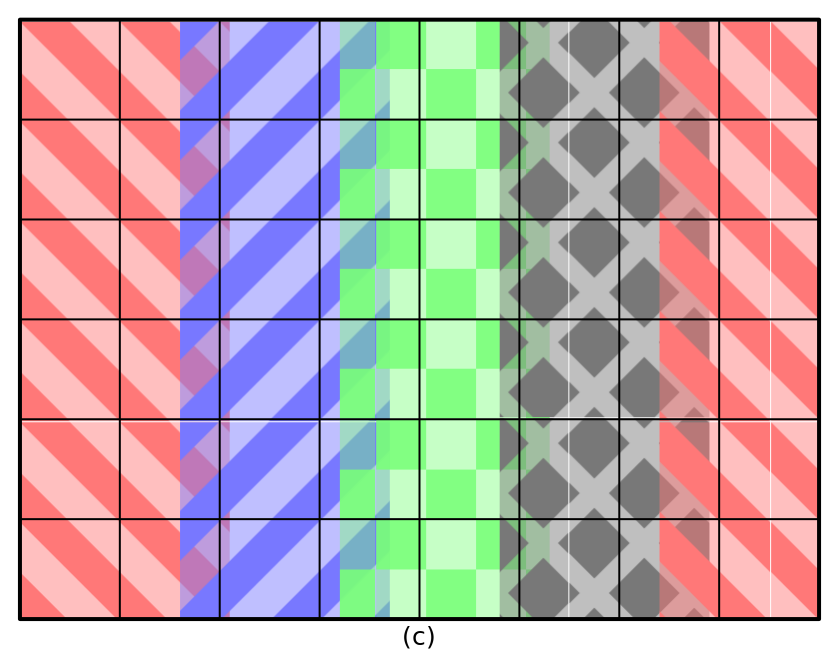
\includegraphics[width=0.5\textwidth]{img/fragmentos5.pdf}
	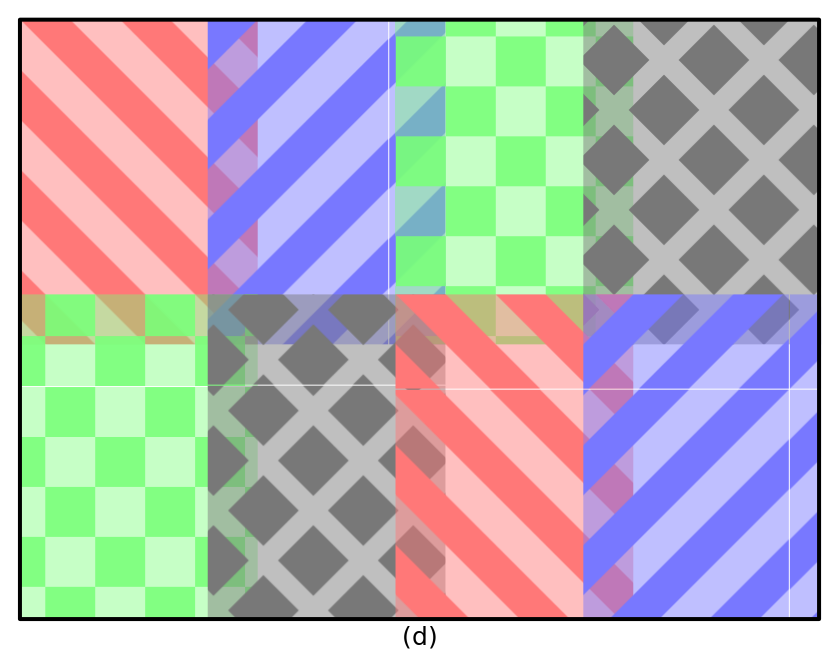
\includegraphics[width=0.5\textwidth]{img/fragmentos8.pdf}
	\caption{Resultado de dividir un cuadro de 800x600 píxeles con un área
	compartida de 50 píxeles en 1(a), 2(b), 5(c) y 8(d) fragmentos.}
	\label{fragmentos}

\end{figure}

\section{Implementación del framework}

\label{implementacionFramework}

Como primera etapa se implemento un famework base que simula el procesamiento de
ítems prototipo vacíos y establece las clases base a ser extendidas. Esto
permite explicar el flujo de la información así como la estructura base del
sistema sin preocuparse por la implementación especifica para el sistema de
visión global para el fútbol de robots.

El framework fue implementado en \emph{C++} con \emph{OpenMP} y está basado en
plugins para facilitar su modificación en un ambiente educativo. La elección del
lenguaje se debe principalmente a su eficiencia y paradigma. Dado que el sistema
debe procesar los cuadros en tiempos acotados, la eficiencia es crucial,
mientras que el paradigma orientado a objetos permite establecer fácilmente la
interfaz de los plugins. El uso de \emph{OpenMP} permite la creación y control
de hilos de ejecución y tareas de forma sencilla. Se utilizaron los plugins
implementados en \cite{torres2014}, modificándolos para permitir su uso en un
sistema paralelo.

En la figura \ref{codigo} se muestra el fragmento de código (en pseudocódigo)
que ejecuta y crea las tareas principales del framework. En la función principal
(\emph{main}, linea 1 a 19) se crean las tareas de generación de cuadros (lineas
6 y 7) y generación de tareas de fragmentación de cuadros (lineas 8 a 10)
utilizando el modelo de \emph{fork and join}. El control de la finalización del
programa se realiza a través de una variable compartida \emph{continuar}.

La tarea de generación de tareas de fragmentación de cuadros se implementa en la
función \emph{generaciónDeTareasDeFragmentaciónDeCuadros} (lineas 23 a 58). La
función comienza estableciendo una región de trabajo compartido bajo el modelo
de tareas, se crean $N+1$ hilos de ejecución (linea 25), $N$ hilos para las
tareas de búsqueda y uno adicional para la tarea de generación de tarea de
fragmentación de cuadros. La tarea de generación de tareas de fragmentación de
cuadros implementa una espera ocupada sobre la cola de cuadros a procesar. La
finalización de la tarea es controlada por la variable \emph{continuar}.

Cuando hay hilos de búsqueda libres y cuadros en la cola de cuadros, se toma un
cuadro de la cola de cuadros (lineas 29 a 32), y se crea una tarea de
fragmentación de cuadro con una copia privada del puntero al cuadro (lineas 33 a
36).

Cada tarea de fragmentación de cuadro (lineas 37 a 53), comienza fragmentando el
cuadro. Por cada fragmento crea una tarea de procesamiento de fragmento (lineas
40 a 43). Cuando la tarea de fragmentación de cuadro finaliza, libera al hilo de
ejecución.

Cada tarea de procesamiento de fragmento (lineas 44 a 52) procesa el fragmento
con cada pila (lineas 45 a 48). Cuando se termina de procesar el fragmento con
todas las pilas se borra el fragmento (linea 49) y se libera el hilo de
ejecución.

\begin{figure}[!h]

	\centering

	\includegraphics[width=0.5\textheight]{img/itemSwitch.pdf}

	\caption{Pseudo código del sistema}

	\label{codigo}

\end{figure}

En la figura \ref{hilosytareas} se muestra una posible secuencia de ejecución.
Dado que el procesamiento de los fragmentos tiene un tiempo variable, los hilos
se liberan de forma irregular, lo que lleva a que el orden de creación de las
tareas para los distintos cuadros no sea completamente determinista.

\begin{figure}[!h]

	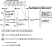
\includegraphics[width=\textwidth]{img/hilosytareas.pdf}

	\caption{Asignación de las tareas a los hilos de búsqueda}

	\label{hilosytareas}

\end{figure}

Las clases del framework básico son las siguientes:

\begin{description}

	\item[Item:] Esta clase define un tipo prototipo de los ítems que serán
		tratados por el sistema. En la implementación especifica para el
		sistema de visión global para el fútbol de robots, los cuadros
		son subclase de la clase \emph{Item}.

	\item[RingBuffer:] Este es el buffer donde se guardan los ítems
		generados mientras esperan ser procesados. El buffer guarda solo
		punteros a objetos de la clase \emph{Item} y no tiene mecanismos
		de control que permitan acceder la estructura desde múltiples
		hilos al mismo tiempo de forma segura. Cuando se solicita un
		ítem, se devuelve el puntero al más antiguo o \textbf{NULL} en
		caso de que la estructura este vacía. Cuando se intenta agregar
		un nuevo ítem pero la estructura esta llena, se coloca este en
		el espacio del ítem más viejo en la estructura y se retorna el
		puntero de este al llamador, delegándole su destrucción. La
		razón de la delegación de la destrucción se debe a que la
		destrucción un objeto es lenta (y aun mayor en el caso de los
		cuadros del sistema final), y el control de acceso al buffer se
		realiza a través del uso de de secciones criticas, por lo que es
		importante reducir el tiempo que cada hilo pasa dentro de la
		sección critica, para no impedirle el acceso a otros hilos que
		pueden estar esperando entrar a ellas.

	\item[Input:] Se trata de una clase que funciona como definición de la
		interfaz de las clases que generan los ítems. Sus métodos
		principales son \emph{run} y \emph{generate}. El método
		\emph{generate} debe ser re implementado por las clases hijas
		para generar el tipo de ítem especifico del sistema. El método
		\emph{run} es el encargado de generar los ítems llamando a
		\emph{generate} y colocarlos en el \emph{RingBuffer}. Este
		último método puede ser redefinido si la aplicación así lo
		requiere.

	\item[ItemSlicer:] Es la clase que define la interfaz de las clases
		encargadas de dividir los ítems. Se definen tres métodos. El
		primero es \emph{slice} que recibe como parámetro un ítem y la
		cantidad de partes en la que este debe ser dividido y retorna un
		arreglo de ítems. Algunos plugins pueden agregar información a
		los fragmentos de los ítems, con el fin de ser utilizada por
		plugins posteriores dentro de la misma pila, es por esto que
		antes de continuar con la siguiente pila se utiliza el método
		\emph{resetItem} que elimina la información agregada por los
		plugins, retornando al fragmento a su configuración inicial. El
		tercer método es \emph{delPart} que recibe como parámetro un
		fragmento de ítem y lo elimina.

	\item[Plugin:] Esta clase define una interfaz para los plugins que
		realizaran las distintas partes del procesamiento de la imagen.
		Solo se define el método \emph{process} que tiene como único
		parámetro un puntero a un objeto de la clase \emph{Item}.

	\item[PluginStack:] Esta es la clase que tomara el ítem y se encarga de
		entregarlo a cada uno de los plugins. Tiene solo dos métodos,
		\emph{addPlugin}, para agregar un plugin, y \emph{process} que
		tiene como parámetro un ítem, para procesarlo.

	\item[ItemSwitch:] Esta es la clase encargada de implementar la tarea de
		generación de tareas de fragmentación de cuadro. Para no crear
		mas tareas de las que puede procesar el sistema, solo se toma un
		cuadro de la cola de cuadros a procesar si hay hilos de búsqueda
		libres (o lo que es lo mismo, la cola de tareas esta vacía).
		Cada tarea de fragmentación de cuadro divide el ítem utilizando
		\emph{ItemSlicer} y crea una nueva tarea de procesamiento de
		cuadros por cada fragmento.

\end{description}

En la figura \ref{clasesFramework} se muestra el diagrama de clases del
framework base.

\begin{figure}[h]

	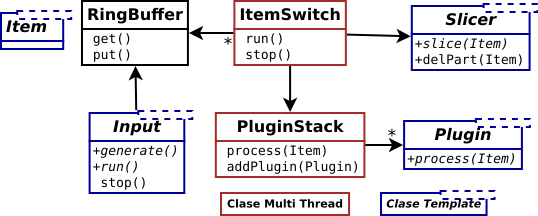
\includegraphics[width=\textwidth]{img/clasesFramework.pdf}

	\caption{Diagrama de clases Framework base.}

	\label{clasesFramework}

\end{figure}

Existen dos parámetros ajustables. El primero es la cantidad de hilos que
ejecutarán las tareas de búsqueda. El segundo parámetro es la cantidad de partes
en las cuales se dividirá el cuadro.

Para extender el framework para utilizarlo como un sistema de visión por
computadora para el fútbol de robots se incorporaron las siguientes clases, las
cuales fueron tomadas y modificadas del sistema de visión presentado en
\cite{torres2014}:

\begin{description}

	\item[Frame:] Subclase de \emph{Item}. Contiene una imagen que
		representa un cuadro y una estructura auxiliar que contiene la
		información necesaria para el funcionamiento de los plugins.

	\item[CaptureFromFile:] Subclase de \emph{Input}. Es la clase encargada
		de crear el flujo de objetos \emph{Frame}, tomando cada cuadro
		desde un archivo de vídeo. También debe respetar la taza de
		cuadros por segundo del vídeo.

	\item[FastCaptureFromFile:] Subclase de \emph{Input}. Muy similar a
		\emph{CaptureFromFile}, con las diferencias de que carga los
		cuadros a memoria antes de que comience el sistema a capturar
		los cuadros (para evitar los retardos de la lectura de disco y
		decodificación), y que tiene dos modos de controlar la
		frecuencia de la generación de los cuadros. Se puede adelantar
		la creación de cuadros si la cola de cuadros a procesar esta
		vacía, o fijar la frecuencia de su creación a un valor
		especifico. Esta clase es útil para comprobar la capacidad
		máxima del sistema, ya que permite simular una cámara con la
		velocidad de captura que se desee, y los distintos modos
		permiten testear la carga máxima en cuadros por segundo
		soportada por el sistema, así como los tiempos de espera bajo
		una cantidad de cuadros por segundo especifica.

	\item[FrameSlicer:] Subclase de \emph{ItemSlicer}. Cada cuadro es
		dividido en rectángulos del mismo tamaño (excepto por los
		cuadros en los bordes inferiores y derechos, que pueden ser
		más pequeños). Cada sub cuadro incluye un área solapada con
		los cuadros adyacentes para asegurar que todos los objetos
		(robots y pelota) se encuentren completamente en por lo menos
		un sub cuadro.

	\item[Subclases de \emph{Plugin}:] \emph{PluginBlur},
		\emph{PluginColorConversions}, \emph{PluginColorSegmentation},
		\emph{PluginDetectBalls}, \emph{PluginFindBlobs},
		\emph{PluginFindSecondariesBlobs}, \emph{PluginMorphology} y
		\emph{PluginNetworking}.

	\item[Clases auxiliares:] \emph{ball}, \emph{colorspace},
		\emph{datastruct}, \emph{homography}, \emph{marker},
		\emph{pattern}, \emph{pattern\_matching},
		\emph{practicalsocket}, \emph{segmentation}, \emph{team},
		\emph{timer}.

\end{description}

En la figura \ref{clasesFrameworkRobots} se muestra el diagrama de clases del
framework extendido para ser utilizado como sistema de visión global para
fútbol de robots.

\begin{figure}[h]

	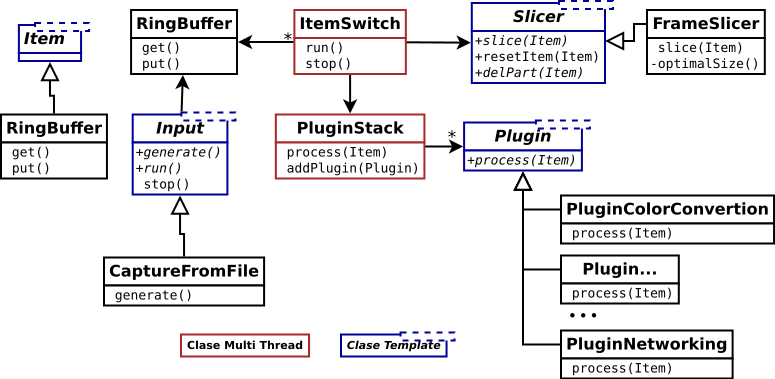
\includegraphics[width=\textwidth]{img/clasesFrameworkRobots.pdf}

	\caption{Diagrama de clases del sistema de visión para el fútbol
	de robots.}

	\label{clasesFrameworkRobots}

\end{figure}

Conceptualmente, la implementación para fútbol de robots tiene dos pilas, una
para búsqueda de robots y la otra para búsqueda de la pelota. Sin embargo, para
ambas pilas los primeros tres plugins realizan la misma tarea de pre
procesamiento (plugins de conversión de color, segmentación de color y
morfología), mientras que los plugins propios de cada pila (para la búsqueda de
la pelota, plugin de búsqueda de pelota. Para la búsqueda de los robots, plugins
de detección de regiones principales y detección de regiones secundarias) no
modifican el cuadro, permitiendo unir ambas pilas en una sola y realizar el pre
procesamiento una vez por cuadro. El plugin de difusión se ejecutara dos veces,
una para enviar los datos de la pelota y otra para enviar los datos de los
robots. En la figura \ref{pilasUnificadas} se muestra la pila de búsqueda
unificada que utiliza el sistema final.

\begin{figure}[h]

	\centering

	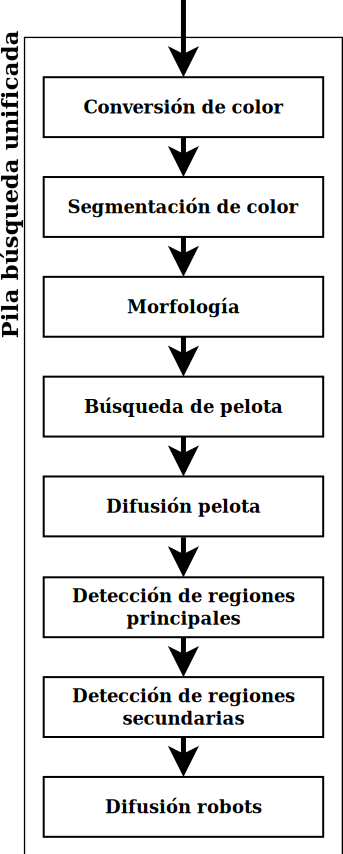
\includegraphics[height=0.25\textheight]{img/pilasUnificadas.pdf}

	\caption{Pila de búsqueda unificada utilizada por el sistema final.}

	\label{pilasUnificadas}

\end{figure}


\chapter{Experimentación}

\label{experimentacion}

% vim: set spell spelllang=es syntax=tex :

\section{Metodología experimental}

\label{metodologiaExperimental}

Para comprobar el funcionamiento del nuevo framework se grabo un vídeo a partir
del cual se crearon dos, uno con una resolución de 800x600 píxeles y otro con
una resolución de 1280x720 píxeles.

Se configuraron diferentes experimentos haciendo variar la cantidad de partes en
las que fueron divididos los cuadros entre 1 y 24, la cantidad de hilos de
ejecución para tareas de búsqueda entre 1 y 12, con ambos vídeos. Para comparar
los resultados de las diferentes configuraciones se midieron los \emph{FPS}
soportados por el sistema y el tiempo de espera máximo (obtenido a los
\emph{FPS} soportados por el sistema bajo la misma configuración).

Se configuraron diferentes experimentos haciendo variar la cantidad de partes en
las que fueron divididos los cuadros y la cantidad de hilos de búsqueda, para
ambos vídeos. Para comparar los resultados de las diferentes configuraciones se
midieron los \emph{FPS} soportados por el sistema y el tiempo de espera máximo
(obtenido a los \emph{FPS} soportados por el sistema bajo la misma
configuración).

Como la obtención del retardo máximo depende del conocimiento previo de los
\emph{FPS}, cada experimento se dividió en dos partes. En la primera parte se
busca la cantidad de \emph{FPS} soportados por el sistema para esa
configuración. Para esto, el programa procesa tantos cuadros del vídeo como
pueda en un cierto intervalo de tiempo. En la segunda parte se limita la
cantidad de cuadros por segundo (según el valor máximo de \emph{FPS} encontrado
en la primera parte del experimento) y se registra el tiempo de espera máximo.
Dado que se trata de un sistema de tiempo real, es importante determinar las
cotas inferiores del rendimiento. Por esto, se repitió cada experimento 10
veces, registrando sólo el peor valor obtenido para cada variable en cada
configuración.

Dada la gran cantidad de experimentos, se buscó el tiempo mínimo de ejecución
necesario para que éstos fueran representativos de una ejecución prolongada. Se
realizaron tres ejecuciones de 6 minutos cada una con una misma configuración:
11 hilos y 10 fragmentos procesando el vídeo de 800x600 píxeles de resolución.
El primer minuto no se contabilizó, con el fin de permitir que la ejecución se
estabilizara. Dado que los 6 minutos de vídeo no caben en la memoria RAM del
equipo de pruebas, el sistema fue modificado para reintroducir en la lista de
cuadros a procesar aquellos cuadros ya procesados. Los resultados se compararon
con ejecuciones utilizando la misma configuración, es decir: utilizando el mismo
framework modificado para reutilizar los cuadros, utilizando 11 hilos, y
dividiendo el vídeo de 800x600 píxeles de resolución en 10 fragmentos, pero
ejecutando de 11 a 20 segundos, y contabilizando sólo los últimos 10 segundos.
El uso del framework modificado para este experimento en particular tiene un
rendimiento menor al framework original, por lo que los resultados son distintos
a los presentados en la sección \ref{resultados} cuando se utiliza la misma
cantidad de fragmentos e hilos. En la tabla 1 se muestran los \emph{FPS}
obtenidos para cada ejecución. Se observa que las pruebas de 16 segundos son
representativas de ejecuciones más largas.

\begin{table}[h]
	\centering
	\begin{tabular}{c||c|c|c|c|c|c|c|c|c|c|c}

		Ejecución&6min&11s&12s&13s&14s&15s&16s&17s&18s&19s&20s\\

		\hline
		\hline

		1&166& 171& 170& 170& 170& 169& 166& 166& 166& 166& 165\\

		\hline

		2&166& 171& 170& 170& 170& 168& 167& 166& 166& 165& 166\\

		\hline

		3&166& 171& 170& 170& 170& 169& 166& 166& 167& 166& 165

	\end{tabular}

	\caption{Búsqueda de la duración mínima de los experimentos}

\label{tabla}

\end{table}

\section{Plataforma experimental}

\label{plataformaExperimental}

El equipo de pruebas cuenta un procesador Intel Xeon E5-2630. Éste es un
procesador de 6 núcleos con multithreading simultáneo de dos vías, una
frecuencia básica de CPU de 2,30GHz y 2,8GHz en modo turbo, 15MiB de memoria
caché L3, 256KiB de caché L2, 32Kib de caché L1 para datos, y 32 KiB de caché L1
para instrucciones. El equipo posee además 16GiB de memoria RAM. La jerarquía de
memoria se muestra en la figura \ref{topoMemoria}.

\begin{figure}[h]

	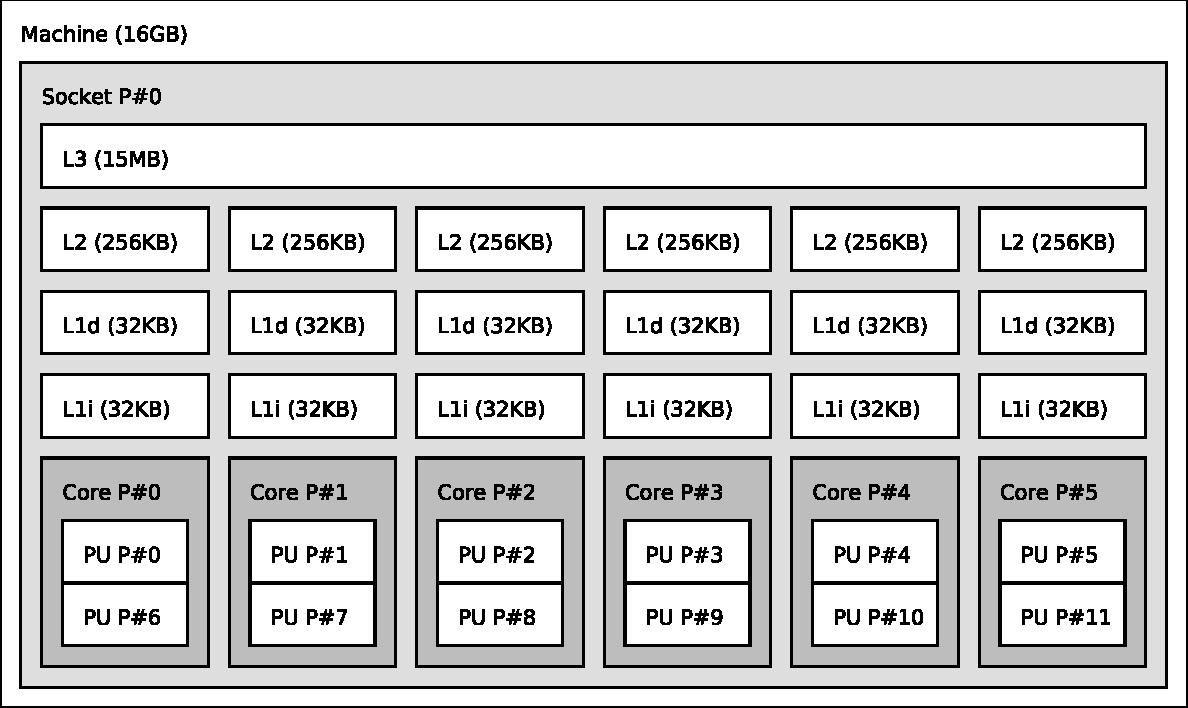
\includegraphics[width=\textwidth]{img/topo.pdf}
	\caption{Jerarquía de memoria de la máquina de pruebas.}

	\label{topoMemoria}

\end{figure}

\section{Diseño de experimentos y resultados}

\label{resultados}

Durante el desarrollo de la aplicación se probaron tres distintas
implementaciones. En la primera implementación, el framework ejecutaba las
distintas pilas de plugins en tareas separadas. En la segunda implementación el
framework fue modificado para que una sola tarea ejecutarán todas las pilas de
plugins sobre un mismo fragmento. Para la tercera implementación se trabajo
sobre el mismo framework que la segunda, pero se unieron las pilas de búsquedas
de robots y la de búsqueda de pelota. Para comprobar cual de éstas era la más
efectiva se realizaron las pruebas con cada una de éstas para la configuración
de 11 hilos de búsqueda y 10 fragmentos con el vídeo de 800x600 píxeles de
resolución. La primera implementación proceso 70 \emph{FPS}, la segunda 152
\emph{FPS} y la tercera 192 \emph{FPS}. Como esta última fue la que produjo
resultados más satisfactorios, sera sobre los resultados de ésta que
trabajaremos a continuación.

El sistema posee 6 núcleos con multithreading simultaneo de dos vías, por lo
cual como máximo puede ejecutar 12 hilos en paralelo. Por este motivo el rango
de la hilos de búsqueda sera inicialmente de 1 a 12 hilos, y en caso de que los
experimentos demuestren que el \emph{speedup} no ha comenzado a decaer, se
extenderá el rango hasta que esto suceda. El rango de cantidad de fragmentos
está limitado de 1 a 24.

En las figuras \ref{800fps} y \ref{1280fps} se muestran las cantidades de
\emph{FPS} alcanzados para un vídeo de 800x600 píxeles y 1280x720 píxeles
respectivamente, para distintas cantidades de hilos de búsqueda y fragmentos.
El número de hilos de búsqueda indica la cantidad de hilos que ejecutan las
tareas de búsqueda. Adicionalmente el sistema ejecuta dos hilos más para las
tareas estáticas, uno para la generación de cuadros y otro para la tarea de
generación de tareas de búsqueda. En el caso de del vídeo de 800x600 píxeles se
llego a un máximo de 196 \emph{FPS} cuando se divide el cuadro en 12 fragmentos
y se utilizan 5 hilos de búsqueda, mientras que para el vídeo de 1280x720
píxeles se alcanzo un máximo de 130 \emph{FPS} cuando se divide el cuadro en 24
fragmentos y se utilizan 10 hilos de búsqueda.

\begin{figure}[h]

	\includegraphics[width=\textwidth]{img/800x600_fps.pdf}
	\caption{FPS alcanzados por el sistema para vídeo de 800x600 píxeles}
	\label{800fps}

\end{figure}

\begin{figure}[h]

	\includegraphics[width=\textwidth]{img/1280x720_fps.pdf}
	\caption{FPS alcanzados por el sistema para vídeo de 1280x720 píxeles}
	\label{1280fps}

\end{figure}

En las figuras \ref{800fps} y \ref{1280fps} se pueden observar dos patrones que
ocurren en ambos vídeos. El primero es que si los cuadros se dividen en 7, 11,
17, 19 y 23 fragmentos, se produce una notable reducción en la cantidad de
cuadros por segundo con respecto a las divisiones adyacentes.

Esto se produce porque cuando los cuadros se dividen en un número primo de
fragmentos, el área total a procesar se incrementa de forma significativa con
respecto a los valores circundantes. En la figura \ref{primosArea} se muestra la
fluctuación de la suma del área de los fragmentos en divisiones de 1 hasta 100
fragmentos para un vídeo de 1280x720 píxeles de resolución, resaltando los
resultados para valores primos y para los valores inmediatamente inferiores y
superiores. Como puede observarse, a partir de 7 fragmentos el área total se
incrementa de forma significativa cuando el número es primo con respecto a los
valores cercanos con divisores. En estos casos, un incremento del número
de fragmentos aumenta el paralelismo, pero es acompañado de un incremento
drástico del área a procesar.

\begin{figure}[h]

	\includegraphics[width=\textwidth]{img/primos_area.pdf}
	\caption{Área total a procesar para número de fragmentos primos y sus inmediatos}
	\label{primosArea}

\end{figure}

Para comprobar como esta variación de volumen de datos afecta la cantidad de
cuadros por segundo procesados, se realizaron nuevas pruebas sobre el vídeo de
1280x720 píxeles de resolución, con 11 hilos de búsqueda y variando la cantidad
de fragmentos entre los números primos mayores a 24 y menores a 100, y sus
inmediatos superior e inferior. Los valores para números primos e inmediatos
inferiores a 24 fueron tomados de los experimentos anteriores. Los resultados
pueden ser observados en la figura \ref{primosFPS}.

\begin{figure}[h]

	\includegraphics[width=\textwidth]{img/primos_fps.pdf}
	\caption{FPS totales para número de fragmentos primos y sus inmediatos}
	\label{primosFPS}

\end{figure}

Como se puede observar en la figura \ref{primosFPS}, para una cantidad de
fragmentos menor a 7, el perjuicio por aumento en el área es menor que el
beneficio aportado por el incremento en el paralelismo. Para cantidades primas
de fragmentos menores a 7, la cantidad de FPS es inferior para la cantidad de
fragmentos inmediatamente anterior, y mayor para la cantidad de fragmentos
inmediatamente posterior. A partir de 7 fragmentos, se produce una reducción de
los FPS si la cantidad de fragmentos es un cantidad prima con respecto las
cantidades de fragmentos inmediatamente anterior y posterior. Si se observa la
figura \ref{primosArea}, dividir el cuadro en 7 fragmentos resulta en el primer
incremento notable de área con respecto tanto a un fragmento menos como un
fragmento más. También se pueden apreciar que los incrementos repentinos en el
área total coinciden con disminuciones repentinas en los cuadros por segundo
procesados.

El segundo patrón que se puede observar en las figuras \ref{800fps} y
\ref{1280fps} es que cuando la cantidad de fragmentos es baja y la cantidad de
hilos de búsqueda es alta, el sistema tiene menor \emph{FPS} que utilizar una
menor cantidad de hilos búsqueda pero una mayor cantidad de fragmentos. La
memoria caché se comparte entre los cuadros que están siendo procesados en
paralelo. Cuanto más cuadros se procesen en paralelo, mayor será la competencia
por la memoria caché. La cantidad de cuadros que se procesan en paralelo está en
relación con el número de fragmentos y la cantidad de hilos de búsqueda.
Considerando que la cantidad de hilos de búsqueda es mayor que la cantidad de
fragmentos, si se disminuye la cantidad de fragmentos, manteniendo la cantidad
de hilos de búsqueda, se incrementa la cantidad de cuadros a procesar en
paralelo. Esto tiene como efecto que los cuadros compitan por la caché y reduce
las posibilidades de que los fragmentos entren completamente en las cachés de
nivel más bajo. Por esto se propuso la hipótesis de que el retardo se produce
debido a un aumento en los fallos de caché.

Para comprobar que la hipótesis es correcta se diseñó el siguiente experimento.
Se ejecutó el programa procesando cuadros del vídeo de 1280x720 píxeles de
resolución, y se midieron los fallos de caché en configuraciones de 1, 2, 3, 4,
6 y 12 fragmentos y cantidad de hilos búsqueda de 1 a 11. Para obtener los
fallos de caché de nivel 3 (es decir, cuando es necesario acceder a datos en la
memoria RAM) se utilizó la herramienta \emph{perf}. Ésta es una aplicación que
permite acceder a los contadores de hardware del procesador que proveen datos
muy precisos con un overhead despreciable.

En la figura \ref{cacheFallos} se muestran los fallos de caché por cuadro
obtenidos en el experimento. En todas las curvas se produce un incremento
significativo de los fallos de cache cuando la cantidad de hilos de búsqueda se
aproxima al doble de la cantidad de fragmentos por cuadro\footnote{Cuando la
cantidad de hilos de búsqueda es el doble de la cantidad de fragmentos por
cuadro, la cantidad de fragmentos que se procesan concurrentemente es la
cantidad contenida en dos cuadros.}.

\begin{figure}[h]

	\includegraphics[width=\textwidth]{img/cache_fallos.pdf}
	\caption{Fallos de caché por cuadro para distintas cantidades de
	fragmentos}
	\label{cacheFallos}

\end{figure}

En las figuras \ref{800turnArround} y \ref{1280turnArround} se muestran los
tiempos máximos de espera de los cuadros, para los vídeos de 800x600 y 1280x720
píxeles de resolución (considerando que los \emph{FPS} son limitados al máximo
encontrado en la primera etapa de los experimentos).

\begin{figure}[h]

	\includegraphics[width=\textwidth]{img/800x600_turnArround.pdf}
	\caption{Tiempos máximos de espera en centésimas de segundo para el
	vídeo de 800x600 píxeles}
	\label{800turnArround}

\end{figure}


\begin{figure}[h]

	\includegraphics[width=\textwidth]{img/1280x720_turnArround.pdf}
	\caption{Tiempos máximos de espera en centésimas de segundo para el
	vídeo de 1280x720 píxeles}
	\label{1280turnArround}

\end{figure}

Estos dos últimas figuras nos permiten apreciar que no siempre una mayor
cantidad de cuadros por segundos procesados implicara el tiempo de espera
mínimo. Dependiendo de si se desea minimizar el tiempo de espera de los cuadros,
maximizar la cantidad de cuadros procesados, o encontrar un balance especifico,
se deberá elegir una cantidad de fragmentos y hilos de búsqueda apropiada. Por
ejemplo, en el caso del vídeo de 1280x720 píxeles de resolución, dividir la
imagen en 24 fragmentos y utilizar 10 hilos de búsqueda permite procesar 130
cuadros por segundo en el equipo de prueba, sin embargo el tiempo de espera es
de $0.28$ segundos. Si el cuadro se divide en 24 fragmentos y se utilizan 12
hilos de búsqueda, la cantidad de cuadros por segundo procesados cae a 128, pero
el tiempo de espera se reduce a $0.09$ segundos. Las figuras \ref{800tFPS} y
\ref{1280tFPS} sintetizan la relación entre los \emph{FPS} y el retardo de
cuadros, mostrando el mínimo retardo de cuadros para los diferentes \emph{FPS}
que puede alcanzar el sistema en cada vídeo.

\begin{figure}[h]

	\includegraphics[width=\textwidth]{img/800x600_tFPS.pdf}
	\caption{Tiempos máximos de espera para vídeo de 800x600 píxeles para
	los FPS soportados por el sistema}
	\label{800tFPS}

\end{figure}

\begin{figure}[h]

	\includegraphics[width=\textwidth]{img/1280x720_tFPS.pdf}
	\caption{Tiempos máximos de espera para vídeo de 1280x720 píxeles para
	los FPS soportados por el sistema}
	\label{1280tFPS}

\end{figure}

Las figuras \ref{bestFPS800} y \ref{bestFPS1280} muestran el máximo rendimiento
en cuadros por segundo obtenidos para cada configuración de hilos de búsqueda
incluyendo el retardo de cuadro, para los vídeos de 800x600 y 1280x720 píxeles.
Se puede apreciar en la figura que para el caso del vídeo de 800x600 píxeles el
sistema escala soló hasta el uso de 5 hilos de búsqueda. En el caso del vídeo de
1280x720 píxeles, también muestra una reducción en el rendimiento cuando se
utilizan 12 hilos de búsqueda. Como la plataforma experimental puede ejecutar
hasta 12 hilos simultáneamente, los hilos de búsqueda deberán compartir recursos
con los hilos dedicados a las tareas estáticas. Por lo cual no podemos
determinar el punto en el cual la aplicación deja de escalar para un vídeo de
1280x720 píxeles, aunque se alcanza un punto de rendimientos decrecientes luego
de los 5 hilos de búsqueda.

\begin{figure}[h]

	\includegraphics[width=\textwidth]{img/800x600_bestfps.pdf}
	\caption{FPS máximos alcanzados para el vídeo de 800x600 píxeles para
	distintas configuraciones de cantidad de hilos de búsqueda. Se incluye
	el retardo de cuadro bajo la configuración y la cantidad de fragmentos
	en la que fue dividido.} \label{bestFPS800}

\end{figure}

\begin{figure}[h]

	\includegraphics[width=\textwidth]{img/1280x720_bestfps.pdf}
	\caption{FPS máximos alcanzados para el vídeo de 1280x720 píxeles para
	distintas configuraciones de cantidad de hilos de búsqueda. Se incluye
	el retardo de cuadro bajo la configuración y la cantidad de fragmentos
	en la que fue dividido.}
	\label{bestFPS1280}

\end{figure}

El \emph{speedup} del rendimiento (sobre los FPS) máximo alcanzado por el
sistema para el vídeo de 800$\times$600 píxeles es de $3.38\times$, mientras que
para el vídeo 1280$\times$720 es de $5.00\times$. Las curvas de \emph{speedup}
son mostradas en las figuras \ref{speedUp800} y \ref{speedUp1280}. Se puede
observar que en ambos casos el crecimiento es pronunciado hasta 6 núcleos, lo
cual corresponde con la cantidad de núcleos físicos de la plataforma
experimental. Existen dos posibles causas para la reducción del crecimiento del
\emph{speedup}. La primera es que con seis hilos de búsqueda se logre suficiente
paralelismo a nivel de instrucción, alcanzando un alto uso de las unidades
funcionales de cada núcleo. La segunda posible causa del decremento del
crecimiento del \emph{speedup} es que la aplicación esté limitada por memoria,
provocando que el acceso a los datos sea cuello de botella, reduciendo el
rendimiento cuando se utilizan más de seis núcleos.

\begin{figure}[h]

	\includegraphics[width=\textwidth]{img/800x600_speedup.pdf}
	\caption{\emph{Speedup} para el vídeo de 800x600 píxeles}
	\label{speedUp800}

\end{figure}

\begin{figure}[h]

	\includegraphics[width=\textwidth]{img/1280x720_speedup.pdf}
	\caption{\emph{Speedup} para el vídeo de 1280$\times$720 píxeles}
	\label{speedUp1280}

\end{figure}


\chapter{Uso educativo}

% vim: set spell spelllang=es syntax=tex :

\section{Uso como herramienta educativa}

\label{usoEducativo}

El sistema puede ser utilizado como herramienta educativa en varios niveles, y
en materias de visión por computadora como materias de sistemas paralelos.

El uso más sencillo que se le puede dar al sistema es simplemente como sistema
de visión global para torneos de fútbol de robots. Dado que ya existe el sistema
utilizado por la \emph{SSL} (llamado \emph{SSL-Vision}), el nuevo sistema sólo
sera útil cuando se necesite un balance especifico de \emph{FPS} y retardo de
procesamiento.

En una materia de sistemas paralelos podría utilizarse el sistema para que los
alumnos experimenten como el varia el rendimiento bajo distintas cantidades de
hilos de búsquedas y particiones en diferente hardware, introduciéndose de esta
manera en las ventajas y limitaciones de los sistemas paralelos. Para este fin
se podrían utilizar las preguntas presentadas a continuación. Algunos valores
deberán ajustadas dependiendo de la plataforma experimental con la que cuenten
los alumnos, en estos ejemplos se considerara que cuentan con la misma
plataforma experimental que de este trabajo.

\begin{enumerate}

	\item{Utilizando el sistema para procesar el vídeo de 800x600 píxeles,
		dividiéndolo el 4 fragmentos:

\begin{enumerate}

	\item{¿Cuantos cuadros por segundo se logran procesar si se utilizan 1 y
		2 hilos de búsqueda?}

	\item{¿Cuantos cuadros por segundo estima que se procesaran
		aproximadamente si se utilizan 3, 4 y 16 hilos de búsqueda?}

	\item{Realice el experimento de procesar el vídeo con 3, 4 y 16 hilos de
		búsqueda ¿Que tan precisa fueron sus predicciones realizadas en
		el inciso anterior?}

	\item{¿Cual espera que sea el comportamiento del sistema si se utilizan
		128 hilos de búsqueda? ¿Y si se utilizan 1024?}

	\item{¿Que explicaciones posibles existen para la reducción del
		\emph{speedup}?}

	\item{Si se tiene una computadora con un procesador de 4 núcleos
		¿Cuantos hilos de búsqueda recomendaría?}

\end{enumerate}}

	\item{Si se utilizan 4 hilos de búsqueda y se dividen los cuadros en 16,
		17 y 18 partes para procesar el vídeo de 800x600 píxeles:

\begin{enumerate}

	\item{¿Cuantos cuadros por segundo procesa el sistema?}

	\item{Limitándose a una cantidad de hilos de búsqueda menor a 17
		¿Encuentra otros valores para los cuales el sistema tenga mayor
		rendimiento tanto si se utiliza un hilo menos o un hilo más?}

\end{enumerate}}

	\item{Utilizando el sistema para procesar el vídeo de 800x600 píxeles:

\begin{enumerate}

	\item{Si se utilizan 12 hilos de búsqueda ¿En cuantos fragmentos deberán
		dividirse los cuadros para que la cantidad de cuadros por
		segundo procesados sea mayor a 180?}

	\item{Si se utilizan 12 hilos de búsqueda ¿En cuantos fragmentos deberán
		dividirse los cuadros para que el retardo del cuadro sea menor a
		6 centésimas de segundo?}

	\item{Si se divide el cuadro en 15 fragmentos ¿Cuantos hilos de búsqueda
		se deberán usar para que la cantidad de cuadros por segundo
		procesados sea mayor a 180?}

\end{enumerate}}

\end{enumerate}

Los plugins del sistema pueden ser modificados tanto en materias de visión por
computadora como en las de sistemas paralelos, pero con enfoques distintos. En
las primeras los alumnos podrían realizar como practica el mejoramiento de la
precisión los plugins, mientras que en la segunda se podría solicitar a los
alumnos que reduzcan los tiempos de los plugins aplicando paralelismo a nivel de
instrucción.

\begin{enumerate}

	\item{Aplicando paralelismo a nivel de instrucción en el plugin de
		segmentación de color reduzca el tiempo de retardo de los
		cuadros.}

\end{enumerate}

Las materias de visión por computadora más avanzadas podrían tener como trabajo
final la implementación de nuevos mecanismos para detectar los robots, pelota, o
nuevos objetos, esto implicaría la creación de nuevos plugins y pilas de
plugins. También se puede plantear como trabajo final adaptar el framework para
un dominio distinto.

\begin{enumerate}

	\item{Para incrementar la detección de infracciones en los partidos de
		la \emph{SSL} se desea agregar un referí a la cancha. Éste es un
		robot similar a los jugadores que proveerá una vista a nivel del
		suelo, se moverá por toda la cancha, y lleva un parche
		cuadriculado blanco y negro. Implemente una nueva pila de
		plugins para la detección del referí.}

	\item{Utilizando como base el framework, implemente un sistema capaz de
		detectar la presencia un marcador de realidad aumentada, su poción y
		orientación con respecto a la cámara, y lo remplace por el logo
		de la \texttt{Universidad Nacional del Comahue} (con la
		orientación correspondiente). El vídeo resultante debe tener un
		retardo menor a un segundo. Puede diseñar su propio marcador de
		realidad aumentada, aunque se recomienda utilizar uno estándar.}

\end{enumerate}


\chapter{Conclusiones y trabajos futuros}

% vim: set spell spelllang=es syntax=tex :

En este capitulo se presentan las conclusiones finales de este trabajo, y se
establecen posibles trabajos futuros.

\section{Conclusiones finales}

\label{concluciones}

En este trabajo se ha presentado un nuevo sistema de visión global por
computadora para el fútbol de robots de la \emph{SSL}, que puede ser utilizado
como herramienta educativa en asignaturas de visión por computadora y sistemas
paralelos, y permite explorar distintas estrategias de paralelización. El
sistema procesa cuadros de video y reporta la posición y orientación de los
robots y la posición de la pelota en cada uno de ellos.

Se describieron dos estrategias de paralelización que son aplicadas en conjunto.
Una de ellas explota el paralelismo dentro de cada cuadro, dividiendo los
cuadros en fragmentos que son procesados de forma independiente. La otra
estrategia se basa en el procesamiento simultáneo de diferentes cuadros del
video (independientes unos de otros).

Se realizó una implementación utilizando el modelo de programación de memoria
compartida \emph{OpenMP} para \emph{C++}, basada en plugins para facilitar su
modificación en un ambiente educativo. Con el fin de sintonizar la aplicación
para extraer el máximo rendimiento de una determinada plataforma hardware, el
sistema cuenta con diferentes parámetros que permiten modificar el
comportamiento de sus estrategias de paralelización. La posibilidad de modificar
el comportamiento de las estrategias de paralelización es útil para que el
estudiante realice experimentación y analice los resultados buscando
explicaciones al impacto en el rendimiento del sistema.

Se estudió el comportamiento del sistema en términos de \emph{FPS} y de retardo
en el procesamiento de los cuadros para diferentes configuraciones del sistema
con videos de distintas resoluciones. Se observó que dividir el cuadro
en un número primo de fragmentos afectaba de forma negativa el desempeño del
sistema, y que un bajo número de fragmentos obliga a los hilos a competir por
los recursos de caché. En un servidor con un procesador Intel Xeon E5-2630 (6
núcleos y multithreading simultáneo) el software es capaz de procesar un video
de 800x600 píxeles de resolución a una taza de 196 cuadros por segundo y un
retardo de procesamiento del cuadro de 318$ms$; y, un video de 1280x720 píxeles
resolución a una taza de 130 cuadros por segundo y un retardo de procesamiento
del cuadro de 113$ms$. Se logro una mejora de 5,42$x$ en los cuadros procesados
por segundo, con respecto a la ejecución del sistema utilizando un único núcleo
(de los 6 disponibles). Esto demuestra que el sistema escala adecuadamente.

Se propusieron ejercicios prácticos que utilizan el sistema como herramienta
didáctica para la enseñanza de visión por computadora y programación de sistemas
paralelos. Ellos se enfocan principalmente en análisis de rendimiento
(\emph{speedup} y eficiencia), impacto de la jerarquía de memoria,
particionamiento de los datos, y programación de plugins y pilas de plugins para
visión por computadora.

\section{Trabajos futuros}

\label{trabajosFuturos}

Si bien el sistema funciona correctamente, existen aspectos que hacen difícil su
aplicación como remplazo para los sistemas de visión global utilizados hoy en
día en las competencias de la \emph{SSL}. En la implementación actual, si se
desea calibrar los colores de los parches o la pelota se deben realizar
modificaciones en el código. Seria deseable una interfaz gráfica que permita
modificar estos datos interactivamente. Seria útil también mostrar gráficamente
la detección de los objetos.

La taza de crecimiento del \emph{speedup} se vio disminuida a partir de los cinco
hilos de búsqueda. Posibles causas son que los accesos a memoria crean un cuello
de botella, o que con cinco hilos de búsqueda se alcanza un alto paralelismo a
nivel de instrucción. Para investigar estas hipótesis podría analizarse la
cantidad de instrucciones por ciclo en cada caso.

Para poder acelerar la búsqueda de los objetos y poder distribuir la carga mas
uniformemente se podría agregar al sistema una base datos de últimas posiciones
conocidas de los objetos. Esto disminuiría la independencia entre los cuadros,
pero tiene el potencial de disminuir drásticamente los tiempos de búsqueda.
Además, se cree conveniente implementar soluciones paralelas optimizadas de los
plugins.



\label{conclucionesYTrabajosFuturos}

\bibliographystyle{plain}

\bibliography{biblio}

\end{document}
